% abtex2-modelo-artigo.tex, v-1.9.2 laurocesar
% Copyright 2012-2014 by abnTeX2 group at http://abntex2.googlecode.com/ 
%
% abnTeX2: Modelo de Artigo Acadêmico em conformidade com
% ABNT NBR 6022:2003: Informação e documentação - Artigo em publicação 
% periódica científica impressa - Apresentação
%-------------------------------------------------------------------------------------------

\documentclass[
	% -- opções da classe memoir --
	article,			% indica que é um artigo acadêmico
	11pt,				% tamanho da fonte
	oneside,			% para impressão apenas no verso. Oposto a twoside
	a4paper,			% tamanho do papel. 
	% -- opções da classe abntex2 --
	%chapter=TITLE,		% títulos de capítulos convertidos em letras maiúsculas
	%section=TITLE,		% títulos de seções convertidos em letras maiúsculas
	%subsection=TITLE,	% títulos de subseções convertidos em letras maiúsculas
	%subsubsection=TITLE % títulos de subsubseções convertidos em letras maiúsculas
	% -- opções do pacote babel --
	english,			% idioma adicional para hifenização
	brazil,				% o último idioma é o principal do documento
	sumario=tradicional
	]{abntex2}

\usepackage{lmodern}			% Usa a fonte Latin Modern
\usepackage[T1]{fontenc}		% Selecao de codigos de fonte.
\usepackage[utf8]{inputenc}		% Codificacao do documento (conversão automática dos acentos)
\usepackage{indentfirst}		% Indenta o primeiro parágrafo de cada seção.
\usepackage{nomencl} 			% Lista de simbolos
\usepackage{color}				% Controle das cores
\usepackage{graphicx}			% Inclusão de gráficos
\usepackage{microtype} 			% para melhorias de justificação
\usepackage{lipsum}				% para geração de dummy text
\usepackage[brazilian,hyperpageref]{backref}	 % Paginas com as citações na bibl
\usepackage[num]{abntex2cite}	% Citações padrão ABNT \alf
\usepackage{authblk}
\usepackage{amsmath}
\usepackage{amsfonts}
\usepackage{multirow}
\usepackage{lscape}
\usepackage{hyperref}
\usepackage{multicol}
\usepackage{geometry}
\usepackage{float}
\usepackage{subcaption}
\usepackage{appendix}

\renewcommand{\backrefpagesname}{Citado na(s) página(s):~}
% Texto padrão antes do número das páginas
\renewcommand{\backref}{}
% Define os textos da citação
\renewcommand*{\backrefalt}[4]{
	\ifcase #1 %
		Nenhuma citação no texto.%
	\or
		Citado na página #2.%
	\else
		Citado #1 vezes nas páginas #2.%
	\fi}%

% Informações de dados

\titulo{IDENTIFICAÇÃO DO PERFIL SOCIO-PSCICOLÓGICO DE USUÁRIOS DE DROGAS}

\author[1]{Albertine Weber}
\author[1]{Eduardo Brock}
\author[2]{Mayara Soares}
\author[2]{Taís Bellini}

\affil[1]{Instituto de Física - Universidade Federal do Rio Grande do Sul}
\affil[2]{Instituto de Matemática e Estatística - Universidade Federal do Rio Grande do Sul}

\local{Brasil}

\data{\today}

% Configurações de aparência do PDF final

\definecolor{blue}{RGB}{41,5,195}
\makeatletter
\hypersetup{
     	%pagebackref=true,
		pdftitle={\@title}, 
		pdfauthor={\@author},
    	pdfsubject={Modelo de artigo científico com abnTeX2},
	    pdfcreator={LaTeX with abnTeX2},
		pdfkeywords={abnt}{latex}{abntex}{abntex2}{atigo científico}, 
		colorlinks=true,       		% false: boxed links; true: colored links
    	linkcolor=blue,          	% color of internal links
    	citecolor=blue,        		% color of links to bibliography
    	filecolor=magenta,      	% color of file links
		urlcolor=blue,
		bookmarksdepth=4
}

\makeatother
\setlrmarginsandblock{3cm}{3cm}{*} % Altera as margens padrões
\setulmarginsandblock{3cm}{3cm}{*} % Altera as margens padrões
\checkandfixthelayout
\makeindex % compila o indice
\setlength{\parindent}{1.3cm} % O tamanho do parágrafo
\setlength{\parskip}{0.2cm}  % Controle do espaçamento entre um parágrafo e outro
\SingleSpacing % Espaçamento simples
%-------------------------------------------------------------------------------------------

\begin{document}
\selectlanguage{brazil}
% ----------------------------------------------------------
% Início da Capa
% ----------------------------------------------------------
    \begin{center}
        \Large
        UNIVERSIDADE FEDERAL DO RIO GRANDE DO SUL\\
        INSTITUTO DE MATEMÁTICA E ESTATÍSTICA\\
        
        \vspace{1.5cm}
 
        Albertine Weber\\
        Eduardo Brock\\
        Mayara Soares\\
        Tais Bellini
        
        \vspace{5.0cm}
        
        \Huge\textbf{ANÁLISE DO PERFIL SOCIO-PSCICOLÓGICO DE USUÁRIOS DE DROGAS}
        
        \vspace{0.5cm}
        
        \LARGE %Subtítulo do Trabalho
        
        \vfill
        
        Projeto final do curso de Machine Learning e Modelagem Estatística ofertado durante o Curso de Verão 2020
 
        \vspace{0.8cm}
 
        \Large
        Porto Alegre\\
        \today
    \end{center}
% ----------------------------------------------------------
% Fim da Capa
% ----------------------------------------------------------
\pretextual
\frenchspacing % Retira espaço extra obsoleto entre as frases.
\maketitle

\begin{resumoumacoluna}
Este trabalho tem como objetivo avaliar os principais fatores que identificam o perfil socio-psicológico de usuários de drogas. Para tal, realizou-se a análise de problemas de classificação quanto ao uso de quatro drogas: álcool, cannabis, ecstasy e um grupo de drogas estimulantes (cocaína, crack e anfetamina). O uso dessas drogas foi avaliado em relação a características sociais e psicológicas dos indivíduos por meio do uso de dois algoritmos de machine learning: regressão logística e árvores de decisão. Os resultados obtidos permitem traçar um perfil para o usuário de drogas com acurácia e sensibilidade consideradas satisfatórias.


 \vspace{\onelineskip}
 
 \noindent
 \textbf{Palavras-chaves}: Uso de Drogas, Machine Learning, Classificação, Regressão Logística e Árvore de Decisão.
\end{resumoumacoluna}

\textual
% ----------------------------------------------------------
% Introdução
% ----------------------------------------------------------
\section{Introdução}

Avaliar o potencial risco do consumo individual de drogas, ilícitas ou não, é um problema de saúde pública: além dos danos que podem ser causados à saúde pelo seu simples uso, as drogas (em particular, as ilícitas) podem implicar em severas consequências para a sociedade, como o surgimento de redes de tráfico ou sujeitando os seus usuários a viverem em condições vulneráveis. Embora muitas vezes as consequências possam ser potencializadas ao indivíduo em questão, o uso de drogas é entendido como um fenômeno não isolado e frequentemente  relacionado a certos grupos comportamentares pelo senso comum \cite{fehrman2015}. Por conta desse fato, muitos estudos tentam abordar o consumo de drogas de forma a identificar quais são esses grupos de risco, de maneira a desenvolver políticas públicas mais direcionadas a esses indivíduos.

Motivados por esse panorama e por considerarmos essa questão relevante para sociedade atual, a modelagem do uso de drogas foi escolhida pelo grupo como temática para o presente trabalho. Nele, iremos abordar diferentes técnicas estatísticas de classificação com o objetivo de encontrar características demográficas e de personalidade dos indivíduos que estejam associadas ao uso de drogas. Para tal, será utilizado um conjunto de dados \cite{dataset_drugs} resultantes de uma pesquisa realizada online sobre o tema, que serviu de base para um extenso trabalho com ênfase na área da psicologia acerca do tema \cite{fehrman2015}.

Serão avaliadas apenas três drogas do conjunto relacionado pela pesquisa, além de um grupo de drogas específicas. As drogas foram escolhidas representando drogas lícitas e ílicitas, sendo elas: álcool, maconha (cannabis), ecstasy e um grupo de drogas estimulantes: cocaína, crack e anfetamina. Para a separação dos grupos, foi observado o desfecho de usuário e não usuário de cada droga, considerandos usuários aqueles que fizeram uso da determinada substância em um período inferior a um ano até o momento da realização da pesquisa.

As análises foram feitas separadamente para cada droga e para o grupo, dado que as distribuições nos atributos estudados pela pesquisa diferem consideravelmente e supondo que diferentes perfis comportamentais podem ser encontrados dependendo da droga avaliada. As técnicas aplicadas foram regressão logística e árvore de decisão, obtendo resultados satisfatórios na faixa dos 70\% de acurácia na classificação. Os modelos resultantes foram avaliados principalmente de acordo com os critérios de acurácia e de sensibilidade: enquanto o primeiro mede a taxa de acerto do ajuste, o segundo mede a capacidade do algoritmo de identificar corretamente os usuários de drogas, que são o foco do trabalho.

% ----------------------------------------------------------
% Cap. 2 - Descrição dos Dados
% ----------------------------------------------------------
\section{Descrição dos Dados}

A base de dados foi coletada a partir de uma pesquisa anônima online, realizada entre março de 2011 e março de 2012. A amostra foi obtida utilizando a amostragem por bola de neve e não foi possível identificar se havia um público alvo definido previamente pela pesquisa. Foram obtidas 2051 respostas,  das quais 166 foram retiradas do banco por estarem mal preenchidas, totalizando 1885 observações restantes. 
A database é constituída por 32 variáveis, sendo a primeira, \emph{ID}, apenas a ordenação da resposta na pesquisa. Dentre as restantes, 12 estão associadas com fatores sociais e comportamentais:

\begin{multicols}{3}
    \begin{itemize}
        \item Idade
        \item Gênero
        \item Educação
        \item País
        \item Etnia

        \item Neuroticismo (N)
        \item Extroversão (E)
        \item Abertura (O)
        \item Socialização (A)
        \item Conscienciosidade (C)

        \item Impulsividade
        \item Busca de Sensações
        \item[]
        \item[]
        \item[]
        
    \end{itemize}
\end{multicols}

As demais 19 variáveis são ligadas ao uso de diferentes drogas. Todos os respondentes classificaram o uso de cada uma das drogas listadas abaixo em 7 possíveis categorias: nunca usou, usou há mais de uma década, usou na última década, no último ano, no último mês, na última semana ou no último dia.

\begin{multicols}{4}
    \begin{itemize}
        \item \textbf{Álcool}
        \item \textbf{Anfetamina}
        \item Nitritos de Alquila
        \item Benzodiazepina
        \item Cafeína

        \item \textbf{Cannabis}
        \item Chocolate
        \item \textbf{Cocaína}
        \item \textbf{Crack}
        \item \textbf{Ecstasy}

        \item Heroína
        \item Ketamina
        \item Legal Highs
        \item LSD
        \item Metadona
        
        \item Cogumelos
        \item Nicotina
        \item Semeron
        \item Inalantes (VSA)
        \item[]
        
    \end{itemize}
\end{multicols}


Uma característica importante de ser ressaltada sobre essa pesquisa é que, devido a forma como a pesquisa foi conduzida, o banco de dados gerado mostrou-se extremamente enviesado. Em sua maioria, as respostas foram de pessoas de nível educacional elevado, brancas e residentes ou do Reino Unido ou dos EUA, e a proporção de usuários de drogas ilegais na amostra é bem mais elevada do que de fato existe entre as populações gerais.

\subsection{Traços de Personalidade (NEO-FFI-R)} \label{neoffir}

A pesquisa utilizou o teste de traços de personalidade NEO-FFI-R, um questionário composto por 60 itens pontuados de 1 (\emph{discordo fortemente}) a 5 (\emph{concordo fortemente}). O questionário permite avaliar as cinco dimensões básicas da personalidade através do modelo de cinco grandes fatores (\emph{Big Five Factors} - modelo amplamente utilizado pela comunidade da área da pscicologia desde a década de 1930): neuroticismo (N), extroversão (E), abertura (O), socialização (A), conscienciosidade (C). A Figura \ref{figura_BigFive} apresenta uma representação esquemática dos cinco fatores, juntamente de alguns comportamentos previstos para pessoas com pontuações altas e baixas associadas a cada fator.

\begin{figure}[H]
    \centering
    \subfloat{{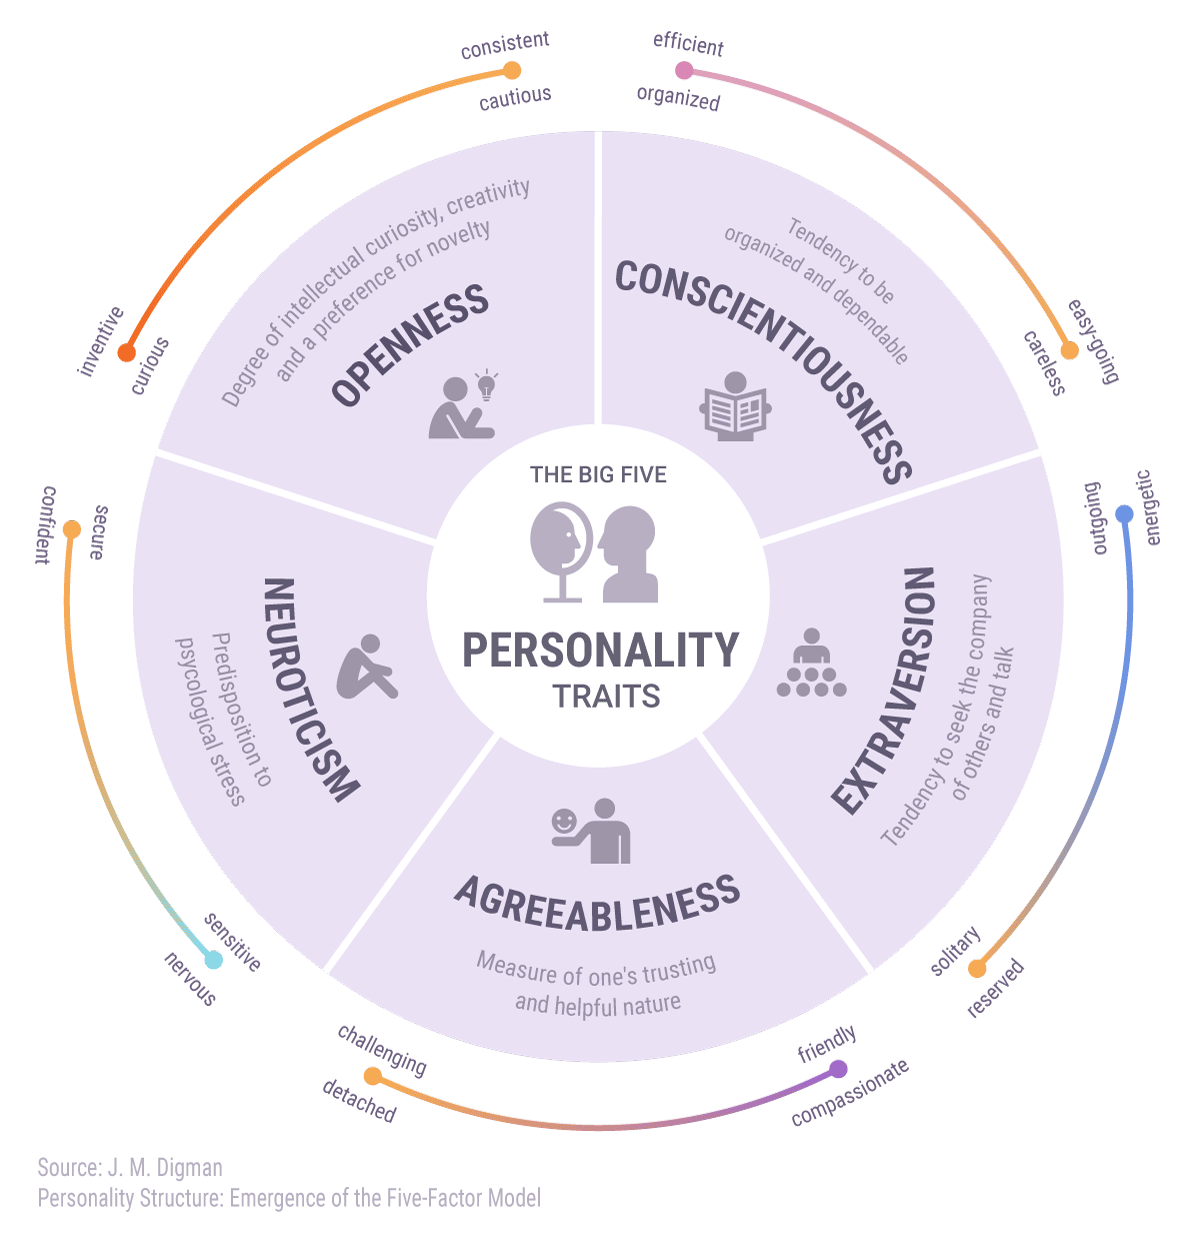
\includegraphics[height=10cm]{figuras/BigFive.png}}}%
    \caption{Os cinco grandes fatores de personalidade}
    \label{figura_BigFive}
\end{figure}

Abaixo uma breve descrição de cada traço de personalidade definido no modelo de cinco grandes fatores, conforme artigo do site \emph{meucerebro.com} \cite{webpage_BigFive}:

\begin{itemize}
    \item \textbf{Neuroticismo (N)} - Mede a instabilidade emocional. Pessoas com pontuações altas nessa escala são ansiosas, inibidas, melancólicas e dotadas de baixa autoestima. Já as que obtém baixa pontuação são de fácil trato, otimistas e dotadas de boa estima consigo mesmas;
    \item \textbf{Extroversão (E)} - É a mais ampla das cinco dimensões. Mede a sensação de bem-estar, o nível de energia e a habilidade nas relações interpessoais. Pontuações elevadas significam afabilidade, sociabilidade e capacidade de se impor. Baixas indicam introversão, reserva e submissão;
    
    \item \textbf{Abertura (O)} - Pessoas com pontuações elevadas gostam de novidades e tendem a ser criativas. Na outra ponta da escala estão os convencionais e ordeiros, os que gostam da rotina e têm senso aguçado do certo e do errado;
    \item \textbf{Socialização (A)} - Refere-se ao modo como nos relacionamos com os outros. Muitos pontos indicam uma pessoa compassiva, amistosa e calorosa. Na outra extremidade estão os retraídos, críticos e egocêntricos;
    \item \textbf{Conscienciosidade (C)} - Mede o grau de concentração. Aqueles com altas pontuações apresentam grande motivação, são disciplinados, comprometidos e confiáveis. Os que apresentam resultados baixos são indisciplinados e se distraem facilmente.
\end{itemize}

Apesar dos Scores possuírem resultados discretos, eles com frequência são agrupados em categorias: scores abaixo de 35 são categorizados como "Very Low", entre 35 e 45 eles são considerados "Low", entre 45 e 55 temos os scores "Average", entre 55 e 65 temos os "High" e acima de 65 possuímos scores na faixa de "Very High".

\subsection{Alterações nos dados}

Os atributos que podem ser utilizados para classificar o uso de drogas são os 12 fatores sociais e comportamentais listados anteriormente. Desses 12, dois atributos, impulsividade e busca por sensações, foram desconsiderados pela falta de embasamento teórico acerca do assunto pelos membros do grupo e de referências confiáveis quanto à classificação dos mesmos. Dessa forma, restam 10 atributos que podem ser divididos em 2 grupos: o grupo de indicadores sociais, composto por Idade, Gênero, Educação, País e Etnia, e o grupo de indicadores comportamentais, composto pelos 5 Scores do NEO-FFI-R (N, E, O, A, C). Para ambos os grupos, analisamos a distribuição de cada variável entre seus diferentes níveis, para decidir se todas as variáveis entrariam na análise e se era necessário alterar algumas categorias.

\subsubsection{Indicadores Sociais}

Os resultados da análise de distribuição para os Indicadores Sociais podem ser observados nas Figuras \ref{soc1}, \ref{soc2} e \ref{soc3}.

\begin{figure}[H]
\centering
\begin{subfigure}{.5\textwidth}
  \centering
  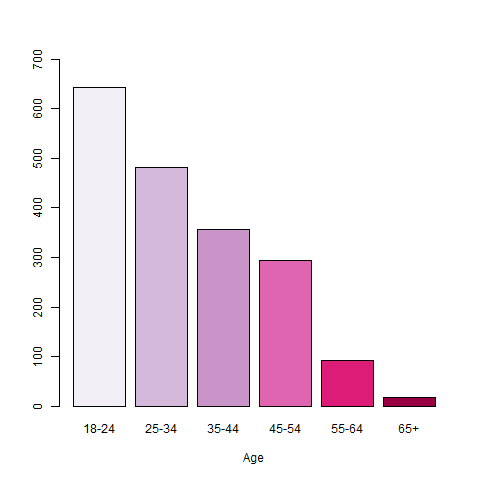
\includegraphics[width=\linewidth]{figuras/dist_idade.png}
  \caption{Distribuição da Variável Age (Idade)}
  \label{soc_idade}
\end{subfigure}%
\begin{subfigure}{.5\textwidth}
  \centering
  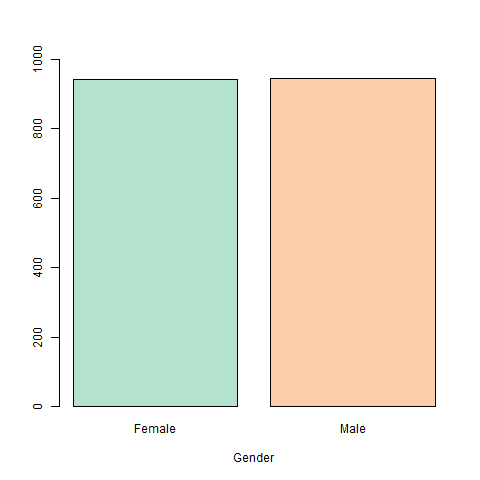
\includegraphics[width=\linewidth]{figuras/dist_genero.png}
  \caption{Distribuição da Variável Gender (Gênero)}
  \label{soc_genero}
\end{subfigure}
\caption{Distribuição dos Indicadores Sociais}
\label{soc1}
\end{figure}

\begin{figure}[H]
\centering
\begin{subfigure}{.5\textwidth}
  \centering
  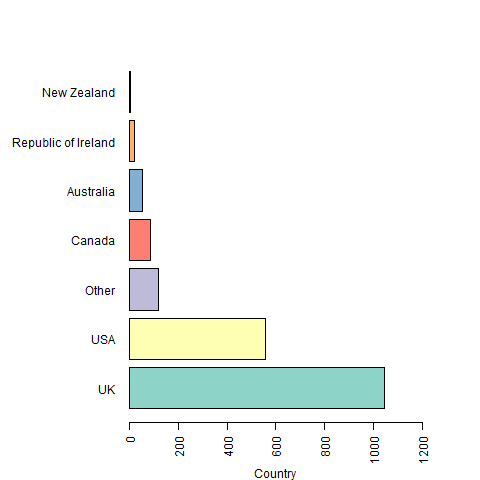
\includegraphics[width=\linewidth]{figuras/dist_pais.png}
  \caption{Distribuição da Variável Country (País)}
  \label{soc_pais}
\end{subfigure}%
\begin{subfigure}{.5\textwidth}
  \centering
  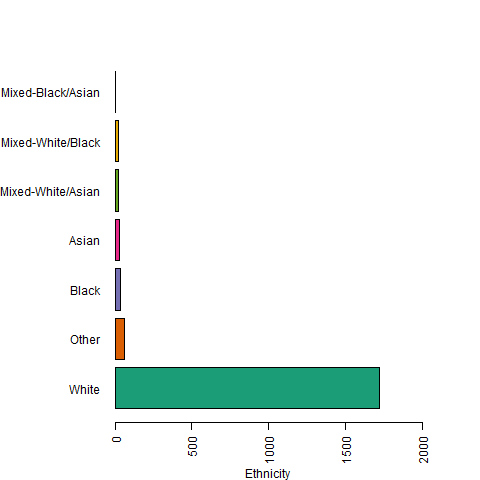
\includegraphics[width=\linewidth]{figuras/dist_etnia.png}
  \caption{Distribuição da Variável Ethnicity (Etnia)}
  \label{soc_etnia}
\end{subfigure}
\caption{Distribuição dos Indicadores Sociais}
\label{soc2}
\end{figure}


\begin{figure}[H]
    \centering
    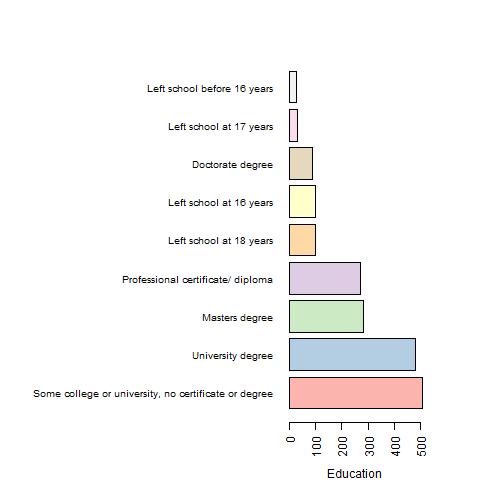
\includegraphics[width=8cm]{figuras/dist_educacao.png}
    \caption{Distribuição do Indicador Social Education (Educação)}
    \label{soc3}
\end{figure}

A partir dessa análise, foi possível observar que dois indicadores sociais apresentavam uma concentração excessiva em categorias específicas: País concentra-se em torno de dois níveis (UK 55\% e USA 30\%), enquanto Etnia está totalmente concentrada no nível "White" (População Branca tem 91\% contra apenas 9\% dos demais). Deste modo, optou-se por retirar a priori ambas as variáveis das análises realizadas, a fim de não prejudicar os resultados obtidos. 

Dos 3 indicadores sociais remanescentes, apenas gênero possui uma distribuição bem balanceada. Para Idade, há uma concentração de índividuos na faixa de 18 a 24 anos e 25 a 34 anos, compondo mais de 50\% da amostra. Na variável educação, observa-se a moda de índividuos na categoria de estudantes sem diploma, com maior concentração de respondentes nas classe de cursos profissionalizantes a diploma de mestrado. Para podermos lidar melhor com essas variáveis, optou-se por agrupar algumas categorias: em Idade, as categorias "45-54", "55-64" e "65+" foram agrupadas de maneira a criarmos a categoria "45+". Para educação, as categorias "Left School before 16 years", "Left School at 16 years", "Left School at 17 years" \hspace{0.05cm} e "Left School at 18 years" \hspace{0.05cm} foram todas agrupadas para criar a categoria "Left School". Além disso, as categorias "Doctorate degree" \hspace{0.05cm} e "Masters degree" \hspace{0.05cm} foram agrupadas na categoria "Graduate degree".

\subsubsection{Indicadores Comportamentais}

Os 5 indicadores comportamentais foram agrupados nas categorias de \textbf{Very Low} até \textbf{Very High} definidas anteriormente na Seção \ref{neoffir} e tiveram suas distribuições observadas. Apesar de eles também apresentarem concentração em torno de algumas categorias específicas, optou-se por não aplicar nenhuma transformação sobre eles, devido ao fato de serem indicadores psicológicos pré-definidos e o grupo não possuir conhecimento suficiente da área para realizar outros agrupamentos. As distribuições de cada Score podem ser observadas nas Figuras \ref{comp1}, \ref{comp2} e \ref{comp3}.

\begin{figure}[H]
\centering
\begin{subfigure}{.5\textwidth}
  \centering
  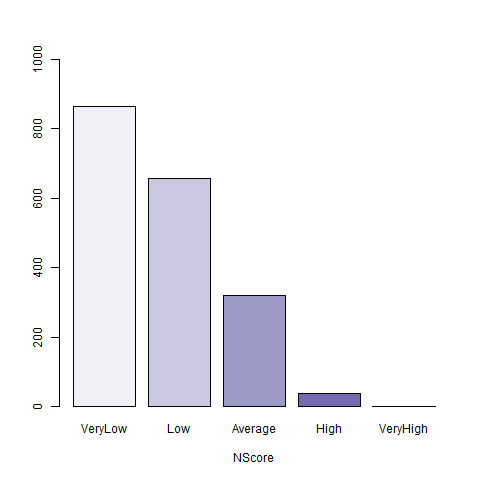
\includegraphics[width=\linewidth]{figuras/dist_nscore.png}
  \caption{Distribuição do NScore (Neuroticismo)}
  \label{nscore}
\end{subfigure}%
\begin{subfigure}{.5\textwidth}
  \centering
  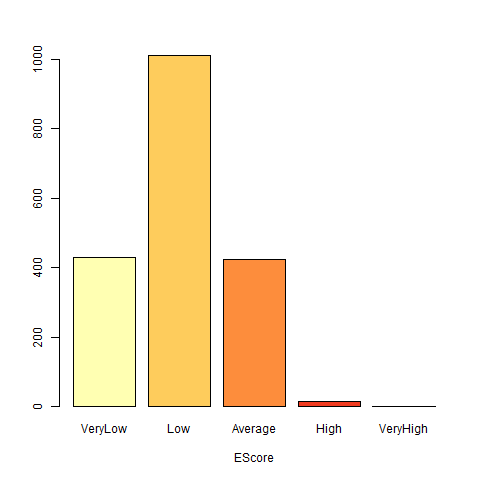
\includegraphics[width=\linewidth]{figuras/dist_escore.png}
  \caption{Distribuição do EScore (Extroversão)}
  \label{escore}
\end{subfigure}
\caption{Distribuição dos Indicadores de Comportamento}
\label{comp1}
\end{figure}

\begin{figure}[H]
\centering
\begin{subfigure}{.5\textwidth}
  \centering
  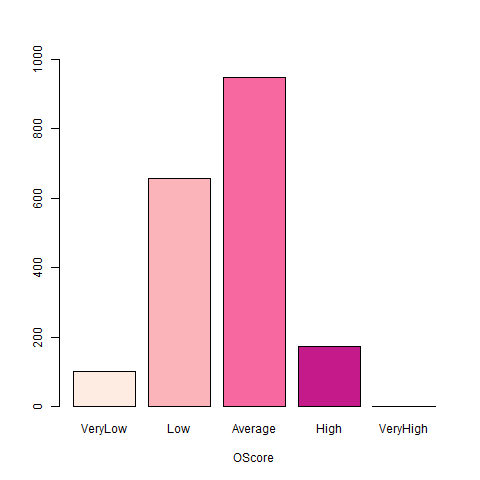
\includegraphics[width=\linewidth]{figuras/dist_oscore.png}
  \caption{Distribuição do OScore (Abertura)}
  \label{oscore}
\end{subfigure}%
\begin{subfigure}{.5\textwidth}
  \centering
  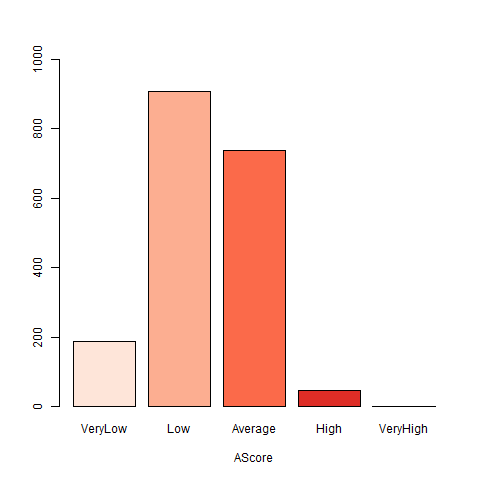
\includegraphics[width=\linewidth]{figuras/dist_ascore.png}
  \caption{Distribuição do AScore (Socialização)}
  \label{ascore}
\end{subfigure}
\caption{Distribuição dos Indicadores de Comportamento}
\label{comp2}
\end{figure}


\begin{figure}[H]
    \centering
    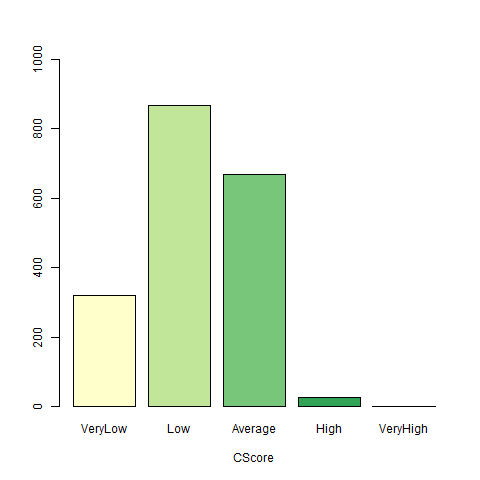
\includegraphics[width=7cm]{figuras/dist_cscore.png}
    \caption{Distribuição do Indicador de Comportamento CScore (Conscienciosidade)}
    \label{comp3}
\end{figure}

\subsubsection{Exclusão de Observações}
Além das transformações nas variáveis, também aplicou-se mudanças nas observações do banco de dados: foram excluídas 8 entradas, pertencentes a usuários que responderam que já haviam utilizado (em qualquer momento) a droga "Semeron". Essa é uma droga fictícia, incluída no estudo justamente para identificar participantes da pesquisa cujas respostas não fossem confiáveis.

\subsubsection{Definição das Variáveis Respostas}
Por fim, a última transformação na base de dados foi realizada em relação às drogas: ao invés de trabalhar com as 19 drogas listadas e com as 7 categorias diferentes de cada uma delas, optou-se por escolher subgrupos para a análise. Em primeiro lugar, decidiu-se trabalhar com um problema de classificação binária - ou seja, apenas classificar se o indivíduo é usuário ou não-usuário de uma certa droga. Para tal, as categorias de \textit{nunca usou}, \textit{usou há mais de uma década} e \textit{usou na útlima década} foram consideradas como "Não Usuários", enquanto as categorias \textit{usou no último ano}, \textit{usou no último mês}, \textit{usou na última semana} e \textit{usou no último dia} foram consideradas como "Usuários". Esse escolha foi feita por considerarmos que a utilização de drogas no período de um ano é uma janela razoável para considerar um indíviduo como usuário, enquanto o período de uma década (que seria o próximo agrupamento possível) já é amplo demais.

Em uma segunda etapa, escolheu-se subconjuntos das 19 drogas para serem analisados. Para tal, realizamos a escolha das drogas baseada em dois critérios: presença razoável de usuários da droga na base (já considerando o período de 1 ano) e popularidade da droga no Brasil (alguma das drogas listadas na pesquisa são mais disseminadas no exterior, sendo pouco conhecidas no Brasil). Dessa forma, foram definidos 4 problemas de classificação diferentes: um envolvendo o uso de uma droga lícita - \textbf{álcool}, um para uma droga ilícita com distribuição bem balanceada - \textbf{maconha}, um para uma droga ilícita com uma distribuição não tão balanceada (70\% - 30\%) - \textbf{ecstasy} e um para um conjunto de drogas agrupadas por possuírem efeito estimulante - \textbf{cocaína}, \textbf{crack} e \textbf{anfetamina}. A distribuição entre usuários e não usuários para cada um desses 4 problemas podem ser observadas nas Figuras \ref{user1} e \ref{user2}.

\begin{figure}[H]
\centering
\begin{subfigure}{.5\textwidth}
  \centering
  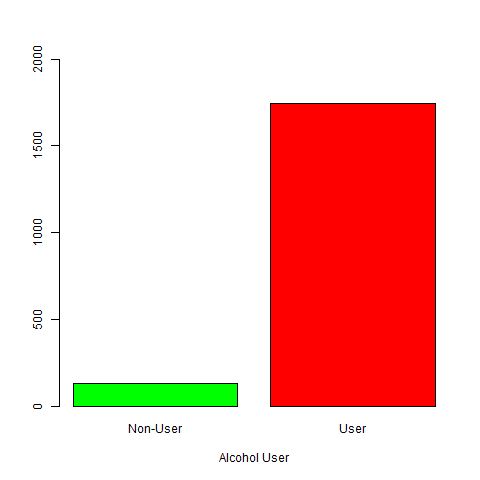
\includegraphics[width=\linewidth]{figuras/dist_user_alcohol.png}
  \caption{Distribuição de Usuários de Álcool}
  \label{distalc}
\end{subfigure}%
\begin{subfigure}{.5\textwidth}
  \centering
  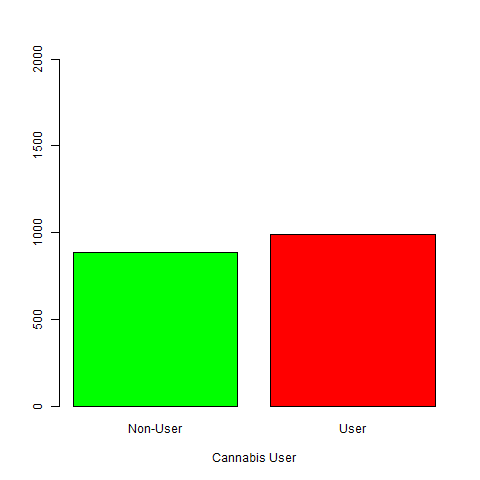
\includegraphics[width=\linewidth]{figuras/dist_user_cannabis.png}
  \caption{Distribuição de Usuários de Maconha (Cannabis)}
  \label{distcan}
\end{subfigure}
\caption{Distribuição de Usuários para as Drogas Selecionadas}
\label{user1}
\end{figure}

\begin{figure}[H]
\centering
\begin{subfigure}{.5\textwidth}
  \centering
  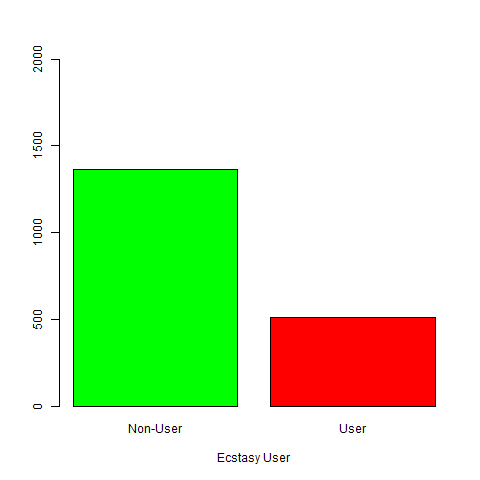
\includegraphics[width=\linewidth]{figuras/dist_user_ecstasy.png}
  \caption{Distribuição de Usuários de Ecstasy}
  \label{distecs}
\end{subfigure}%
\begin{subfigure}{.5\textwidth}
  \centering
  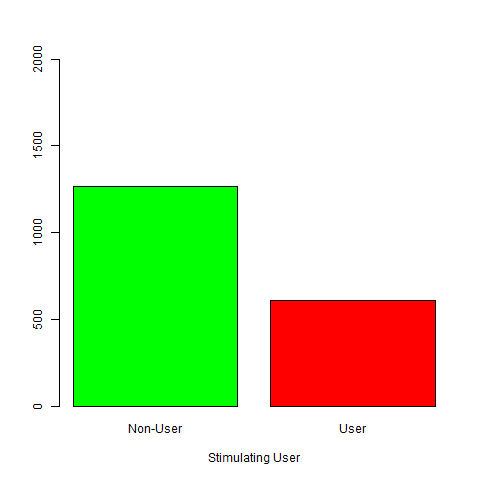
\includegraphics[width=\linewidth]{figuras/dist_user_stimulating.png}
  \caption{Distribuição de Usuários do Grupo de Drogas Estimulantes}
  \label{diststim}
\end{subfigure}
\caption{Distribuição de Usuários para as Drogas Selecionadas}
\label{user2}
\end{figure}

\subsection{Resumo dos dados}

Ao final de todo esse processo de transformações, obtivemos uma base de 1877 observações de 12 variáveis, sendo 8 delas atributos (3 indicadores sociais - Idade, Gênero, Educação - e 5 indicadores comportamentais - Neuroticismo (N), Extroversão (E), abertura (O), Socialização (A) e Conscienciosidade (C)) e 4 respostas sobre o uso de diferentes drogas - álcool, maconha (cannabis), ecstasy e o grupo de drogas estimulantes, composto por cocaína, crack e anfetamina.

Nos Apêndices A e B são apresentadas duas tabelas descritivas dos respondentes da pesquisa, mostrando as frequências e proporções de cada classe considerando o desfecho para cada droga e para o grupo de drogas e já considerando todas as transformações realizadas.



% ----------------------------------------------------------
% Cap. 3 - Métodos Utilizados
% ----------------------------------------------------------

\section{Métodos Utilizados}

O objetivo desde estudo é criar um classificador que, baseado nas variáveis descritas no capítulo 2, indentifique a qual grupo este indivíduo pertence, se usuário ou não de determinada droga ou do grupo de drogas.

Foram avaliados 2 métodos de classificação: Regressao Logística e Árvore de Decisão. 
Em cada método, para cada droga ou grupo de drogas, foi avaliada a possibilidade de reduzir o número de variáveis independentes de forma a manter ou melhorar o resultado. Os modelos finais de cada método serão apresentados e analisados, visando identificar perfis de usuários. Ao final, serão comparados os métodos para definir qual será melhor de acordo com as métricas acurácia e sensibilidade. 

Para ambos os métodos, dividimos a amostra em treino (85\% das observações) e teste (15\% das observações) utilizando a função \textbf{createDataPartition} do pacote \textbf{caret} para garantir distribuições similares. A semente utilizada nessa separação foi 205650. Os códigos detalhados de todos os métodos aplicados podem ser conferidos no repositório do Github utilizado pelo grupo \cite{github}.

\subsection{Regressão Logística}

 Considerando o interesse em avaliar o desfecho dicotômico de usuários e não usuários, e buscando entender a relação entre a variável resposta e as demais variáveis independentes, optou-se por utillizar regressão logística. Este é um método comumente aplicado a esse tipo de modelagem \cite{logreg} já que resulta na probabilidade do indivíduo pertencer a um determinado grupo, neste caso, o de usuários de uma ou mais drogas.
 
 Na estimação e avaliação do modelo através da regressão logística, foi utilizado o método \emph{stepwise backward} para selecionar as variáveis significativas para a predição. O critério utilizado para a seleção foi o AIC, que considera a qualidade do modelo e a simplicidade do modelo. Em alguns casos, atribuiu-se pesos às observações para buscar melhores resultados quando a amostra possuía uma distribuição desbalanceada de usuários e não usuários. Outro ajuste testado, para buscar melhor acurácia e sensibilidade, foi a alteração do ponto de corte da probabilidade predita ao classificar os indivíduos como usuários ou não usuários. 

Na implementação do método, foi utilizado o pacote \textbf{glm} do R, que executa uma gama de modelos lineares, com o parâmetro \emph{family} como \emph{binomial} identificando a regressão logística.
Para cada droga ou grupo de droga, inicialmente, gerou-se um modelo utilizando todas as variáveis e obteve-se acurácia e sensibilidade. Em seguida, foi aplicada a função \textbf{stepAIC} do pacote \textbf{MASS} com o parâmetro \emph{backward} para identificar o método para a seleção de variáveis. No caso das drogas ecstasy, álcool e o grupo de drogas estimulantes, foi adicionado o parâmetro \emph{weight} para buscar melhores resultados em amostras desbalanceadas. As tabelas de \textit{odds ratio} dos modelos ajustados podem ser encontradas no Apêndice C.

\subsection{Árvore de Decisão}

O modelo de Árvores de Decisão é um dos mais simples e intuitivos métodos de classificação através de Machine Learning. Focado na interpretabilidade do ajuste, as árvores de decisão possuem esse nome devido ao fato da representação visual do seu processo decisório se assemelhar com a estrutura de uma árvore. Partindo de um único ponto inicial, esse algoritmo busca classificar uma variável por meio de um conjunto de atributos que são utilizados para gerar uma sequência de ramificações, de tal forma que no final de cada ramo esteja a classe escolhida.

Apesar de ser um método com menor capacidade preditiva e com menos robustez do que vários dos demais algoritmos conhecidos de Machine Learning, as árvores de decisão possuem um papel importante quando realizamos análises focadas em inferência, pois permitem a criação de um modelo de fácil compreensão e interpretação. Além disso, as árvores de decisão se destacam por serem um dos métodos que melhor lidam com a presença de atributos categóricos entre os dados. Por fim, elas possuem uma representação gráfica mesmo quando estamos trabalhando com dimensões maiores do que 3, uma proeza dificilmente alcançada pela grande maioria dos modelos. 

Dessa forma, o uso desse método é facilmente justificável no presente trabalho: estamos em busca de um modelo que permita interpretações e possuímos um conjunto de dados inteiramente constituído por variáveis categóricas. Para aplicá-los, foi usado o pacote \textbf{rpart} do R, que implementa ideias do modelo conhecido como CART (Classification and Regression Tree), descrito em 1984 por Breiman, Friedman, Olshen e Stone \cite{rpart}. Nessa abordagem, a árvore começa a ser construída a partir da variável que melhor separa os dados em dois grupos - melhor separação, aqui, é definida como a ramificação que maximiza a redução da impureza (medida de heterogeneidade) do nó segundo algum critério (em geral, Índice de Gini ou Índice de Informação). Após essa primeira separação, essas etapas são repetidas separadamente para cada subgrupo gerado. O processo segue de forma recursiva até não haver mais melhorias a serem feitas ou até que os subgrupos atinjam um tamanho mínimo. Nesse ponto, a árvore final é gerada. A partir dela, ainda é possível aplicar um procedimento de validação cruzada para podá-la, reduzindo ainda mais o seu tamanho e a sua complexidade.

Assim, aplicou-se o procedimento acima para as drogas escolhidas utilizando-se a função \textbf{rpart} com o Índice de Gini e tamanho mínimo dos subconjuntos como 20 observações. Obteve-se, assim, as matrizes de confusão e as medidas de acurácia, sensibilidade e especificidade do ajuste, além de uma figura representativa da árvore criada. Em todos os casos, as árvores geradas foram posteriormente podadas utilizando-se a função \textbf{prune} e escolhendo-se o parâmetro de complexidade de tal forma que ele estivesse associado ao menor error da validação cruzada que cumprisse a condição (erro relativo + desvio padrão da vaidação cruzada) < erro da validação cruzada. No caso de ecstasy e estimulantes, testou-se ainda o uso de uma matriz de perda que desse mais ênfase na classificação correta de usuários para corrigir o problema de amostras desbalanceadas.

Em todas as figuras geradas para as árvores de decisão, foi necessário alterar o rótulo das variáveis para que eles fossem mais curtos. Para a variável Educação, os códigos utilizados foram: \texttt{Left school = LS16, Some college or university, no certificate or degree = Uwodg, Professional certificate/diploma = Pct, University degree = Udg, Graduate degree = Gdg}. Para a variável Gênero, utilizamos \texttt{Male = M, Female = F}. Para Idade,usamos \texttt{18-24 = J,25-34 = A1, 35-44 = A2, 45+ = MI+}. Para os Scores, utilizamos \texttt{VeryLow = VL, Low = L, Average = A, High = H, VeryHigh = H}.


% ----------------------------------------------------------
% Cap. 4 - Resultados
% ----------------------------------------------------------

\section{Resultados}

% ----------------------------------------------------------
% 4.1 - Cannabis
% ----------------------------------------------------------

\subsection{Cannabis}

A distribuição de usuários e não usuários de maconha é bem balanceada, sendo 52\% usuários, portanto, não foi necessário fazer um ajuste de pesos ou penalidades. 

\subsubsection{Regressão Logística}

As variáveis selecionadas pelo método \emph{stepwise backward} foram: \textbf{Idade (Age), Gênero (Gender), Educação (Education), Conscienciosidade (CScore), Abertura (OScore) e Neuroticismo (NScore)}. 

Os coeficientes estimados pelo modelo podem ser visualizado na Tabela \ref{coef_reglog_cannabis}.

\begin{table}[H]
\centering
\begin{tabular}{|l|r|}
\hline
Intercept                                                     & 0.3924 \\ \hline
Age25-34                                                      & -1.033 \\ \hline
Age35-44                                                      & -1.7719 \\ \hline
Age45+                                                        & -2.2643 \\ \hline
GenderMale                                                    & 0.9081  \\ \hline
EducationLeft school                                          & 1.3836  \\ \hline
EducationProfessional certificate/ diploma                    & 0.7641  \\ \hline
EducationSome college or university, no certificate or degree & 1.254  \\ \hline
EducationUniversity degree                                    & 0.4658 \\ \hline
NScoreHigh                                                    & -0.7821 \\ \hline
NScoreLow                                                     & -0.3322 \\ \hline
NScoreVeryLow                                                 & -0.4299 \\ \hline
CScoreHigh                                                    & 0.0837 \\ \hline
CScoreLow                                                     & 0.6388  \\ \hline
CScoreVeryLow                                                 & 1.0756  \\ \hline
OScoreHigh                                                    & 0.9083  \\ \hline
OScoreLow                                                     & -1.074 \\ \hline
OScoreVeryLow                                                 & -2.116 \\ \hline
\end{tabular}
\caption{Coeficientes da Regressão Logística para a Cannabis}
\label{coef_reglog_cannabis}
\end{table}


A tabela \ref{tabela_RegLogCannabis} apresenta a matriz de Confusão do modelo no conjunto de treino considerando apenas as variáveis selecionadas e utilizando o ponto de corte em 0,5. A acurácia do modelo foi de 76,46\% , a sensibilidade 67,50\% e a especificidade 86,47\%.

\begin{table}[H]
\centering
\begin{tabular}{cc|c|c|c}
\cline{3-4}
 & & \multicolumn{2}{c|}{Valor Verdadeiro} & \\ \cline{3-4}
 & & Positivo & Negativo & \\ \cline{1-4}
\multicolumn{1}{|c|}{\multirow{2}{*}{\rotatebox[origin=c]{90}{Valor Predito}}} & \multicolumn{1}{c|}{\rotatebox[origin=c]{90}{ Positivo }} & \multicolumn{1}{c|}{569} & 102 & \\ \cline{2-4}
\multicolumn{1}{|c|}{} & \multicolumn{1}{c|}{\rotatebox[origin=c]{90}{ Negativo }} & \multicolumn{1}{c|}{274} & 652  & \\ \cline{1-4}
\end{tabular}
\caption{Matriz de confusão da regressão logística no conjunto de treino para a droga cannabis.}
\label{tabela_RegLogCannabis}
\end{table}

Observa-se no gráfico da Figura \ref{fig_LogRegCannabisTrain} que, reduzindo o ponto de corte, é possível obter menos falsos negativos. Isso possibilita aumentar a sensibilidade, que é a métrica de interesse do estudo, pois indica a probabilidade do algoritmo classificar um usuário corretamente. 

\begin{figure}[H]
    \centering
    \textbf{Probabilidade predita e classe verdadeira}\par\medskip
    \subfloat{{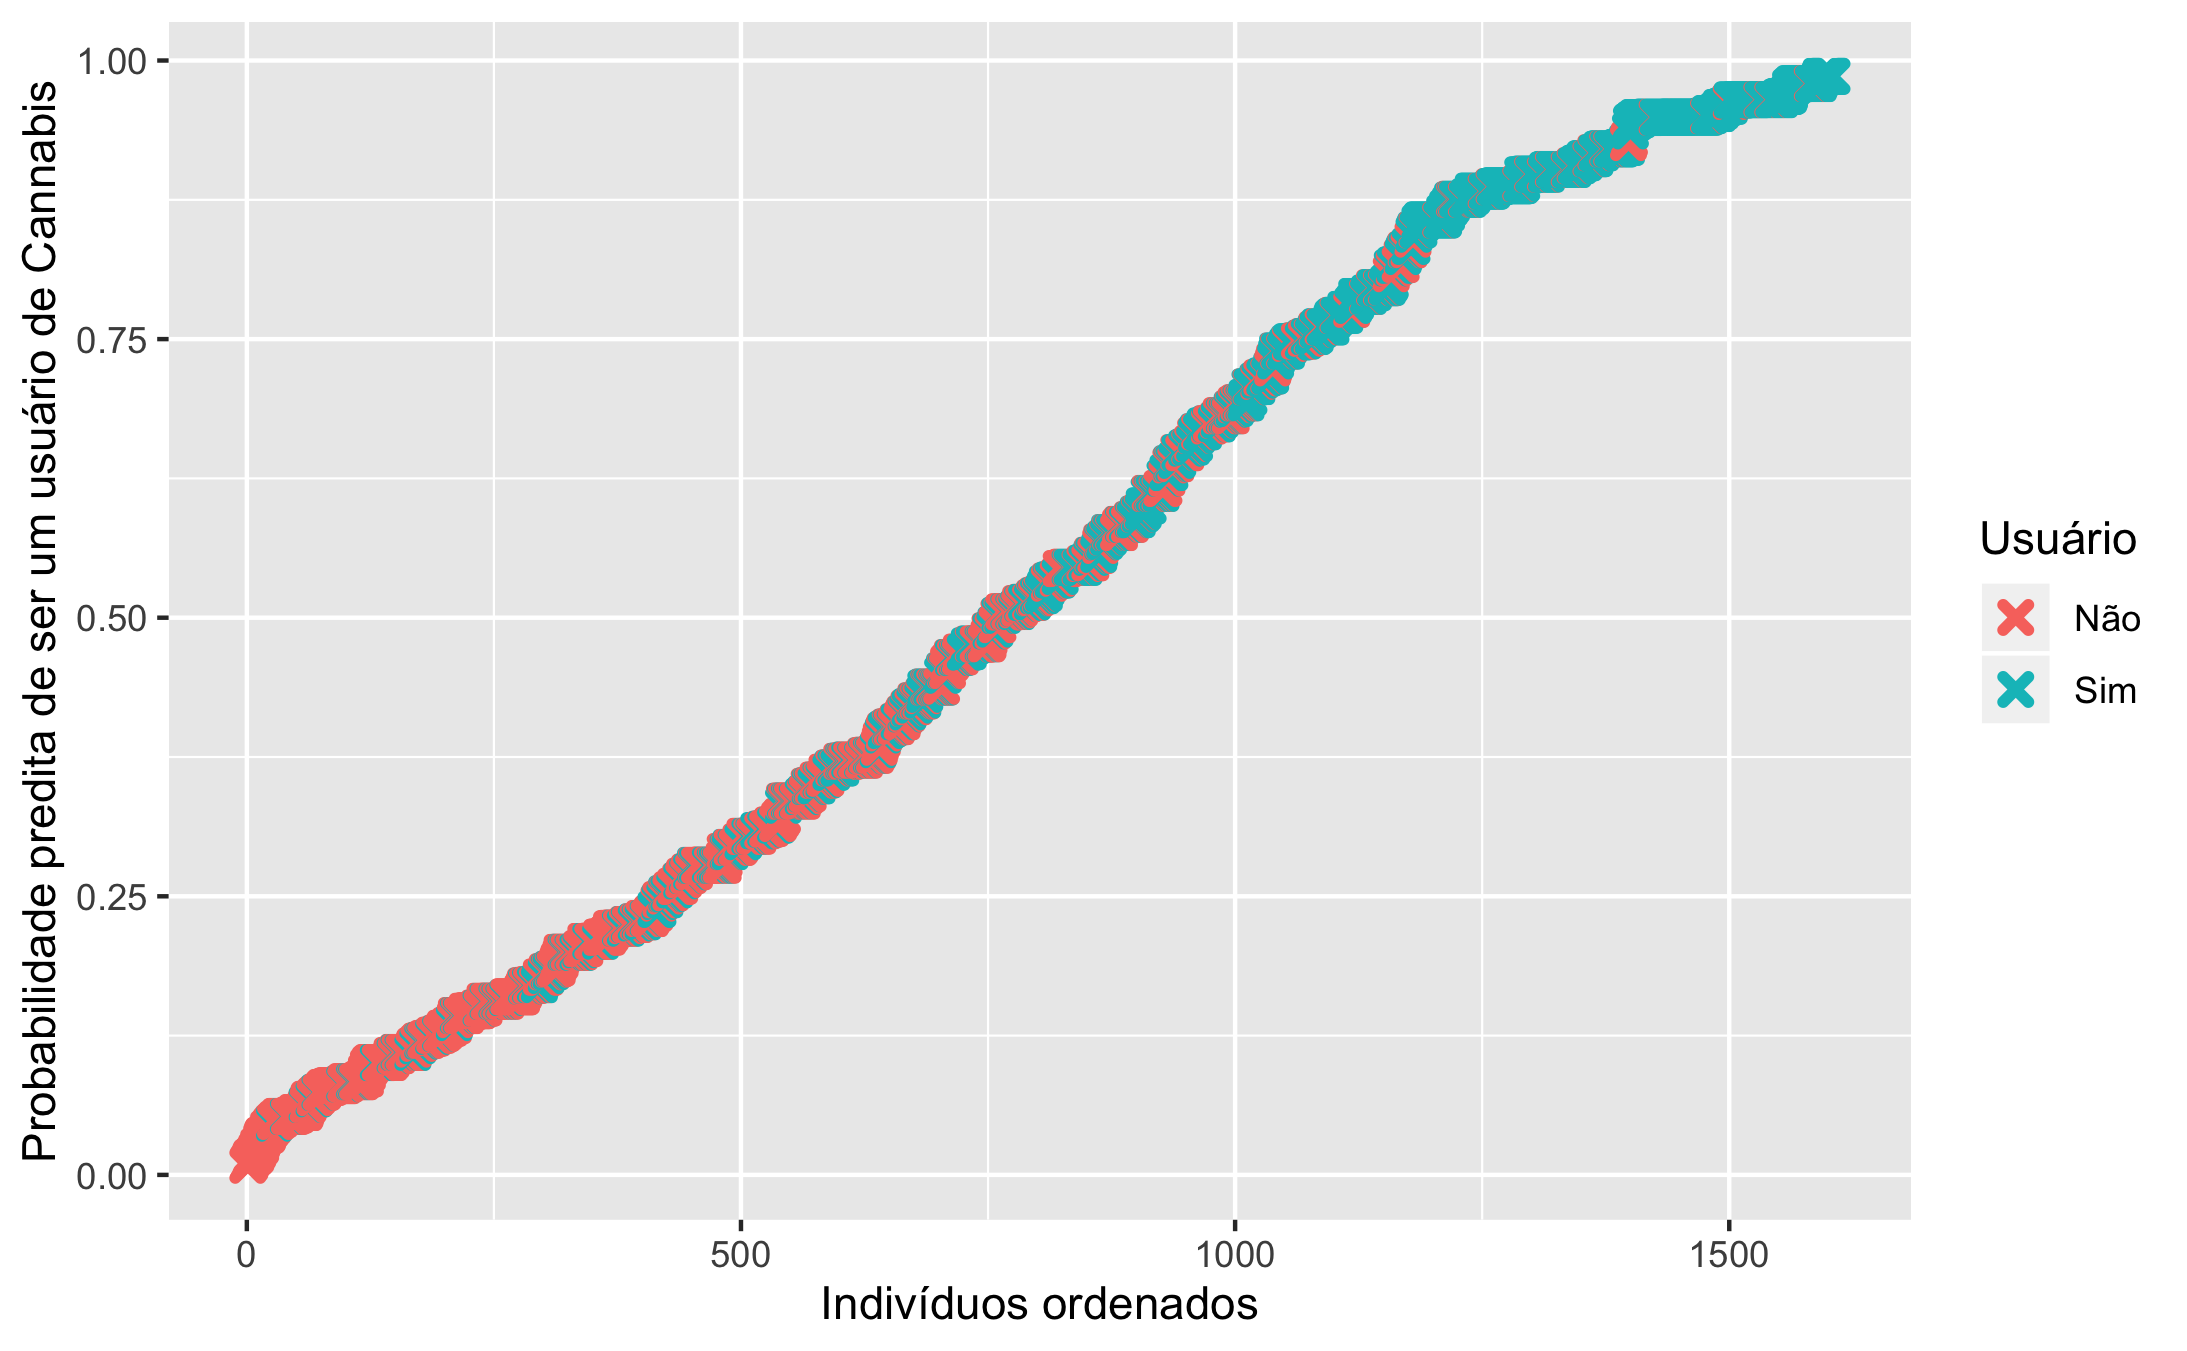
\includegraphics[width=13cm]{figuras/LogRegCannabis.png}}}%
    \caption{Gráfico da probabilidade predita e respectiva classe das observações dos usuários de maconha}
    \label{fig_LogRegCannabisTrain}
\end{figure}

Optando por um ponto de corte de 0,3, tem-se que, ao classificar como usuários indivíduos com probabilidade predita acima de 0,3, há um aumento da sensibilidade para 71,41\%, aumentando a acurácia para 77,27\%, mas com redução na especificidade (83,82\%), como pode ser observado na Tabela \ref{tabela_RegLogCannabis03}. Como o interesse é avaliar as duas primeiras medidas, considera-se que a classificação utilizando este ponto de corte é mais adequada. 

\begin{table}[H]
\centering
\begin{tabular}{cc|c|c|c}
\cline{3-4}
 & & \multicolumn{2}{c|}{Valor Verdadeiro} & \\ \cline{3-4}
 & & Positivo & Negativo & \\ \cline{1-4}
\multicolumn{1}{|c|}{\multirow{2}{*}{\rotatebox[origin=c]{90}{Valor Predito}}} & \multicolumn{1}{c|}{\rotatebox[origin=c]{90}{ Positivo }} & \multicolumn{1}{c|}{602} & 122 & \\ \cline{2-4}
\multicolumn{1}{|c|}{} & \multicolumn{1}{c|}{\rotatebox[origin=c]{90}{ Negativo }} & \multicolumn{1}{c|}{241} & 632 & \\ \cline{1-4}
\end{tabular}
\caption{Matriz de confusão da regressão logística no conjunto de treino para a droga cannabis com ponto de corte em 0,3.}
\label{tabela_RegLogCannabis03}
\end{table}

Aplicando os ajustes escolhidos no conjunto de teste, observa-se que os valores de acurácia, sensibilidade e especificidade ficaram próximos. A sensibilidade aumentou para 75\%, a acurácia se manteve muito próxima (76,43)\% e especificidade reduziu para 78,03\%, como observado nas Tabelas \ref{tabela_RegLogCannabisTeste} e \ref{resultadosreglog_maconha}. 

\begin{table}[H]
\centering
\begin{tabular}{cc|c|c|c}
\cline{3-4}
 & & \multicolumn{2}{c|}{Valor Verdadeiro} & \\ \cline{3-4}
 & & Positivo & Negativo & \\ \cline{1-4}
\multicolumn{1}{|c|}{\multirow{2}{*}{\rotatebox[origin=c]{90}{Valor Predito}}} & \multicolumn{1}{c|}{\rotatebox[origin=c]{90}{ Positivo }} & \multicolumn{1}{c|}{111} & 29 & \\ \cline{2-4}
\multicolumn{1}{|c|}{} & \multicolumn{1}{c|}{\rotatebox[origin=c]{90}{ Negativo }} & \multicolumn{1}{c|}{37} & 103 & \\ \cline{1-4}
\end{tabular}
\caption{Matriz de confusão da regressão logística no conjunto de teste para a droga cannabis com ponto de corte em 0,3.}
\label{tabela_RegLogCannabisTeste}
\end{table}

\begin{table}[H]
\centering
\begin{tabular}{||c|c|c|c||}
\hline
Conjunto & Acurácia & Sensibilidade & Especificidade \\ \hline
Treino (corte 0,5) & 76,46\% & 67,50\% & 86,47\% \\ \hline
Treino (corte 0,3) & 77,27\% & 71,41\% & 83,82\% \\ \hline
Teste (corte 0,3) & 76,43\% & 75,00\% & 78,03\% \\ \hline
\end{tabular}
\caption{Métricas de performance da regressão logística para a droga cannabis.}
\label{resultadosreglog_maconha}
\end{table}

Avaliando os valores \emph{odds ratio} das variáveis, há a indicação de que pessoas com idade acima de 45 anos possuem 90\% menos chance de serem usuárias quando comparadas com pessoas entre 18 e 24 anos. Ainda, percebe-se que indivíduos com alto \emph{score} na característica de personalidade Abertura (O) possuem 2,48 vezes mais chance de serem usuários do que os com \emph{score} mediano e os com \emph{score} muito baixo na característica Conscienciosidade (C) 2,93 vezes mais. É interessante ressaltar também que a chance é 3,99 vezes maior de uma pessoa ser usuária de maconha ao parar de estudar aos 18 anos ou menos do que quem possui um diploma de pós graduação.

\subsubsection{Árvore de Decisão}

Aplicando-se a função \textbf{rpart}, obteve-se um modelo com as seguintes variáveis: \textbf{Idade (Age), Conscienciosidade (CScore), Gênero (Gender), Abertura (OScore)}. O modelo foi capaz de obter acurácia, sensibilidade e especificidade consideravelmente altas tanto para o conjunto de treino quanto o de teste, com todas as métricas ficando acima dos 70\%. Esses resultados podem ser observados em maiores detalhes nas Tabelas \ref{resultadosdt_maconha} e \ref{matrizconfusaodt_maconha}. Uma visualização do processo decisório da árvore produzida pode ser observada na Figura \ref{fig_DTCannabis}.

\begin{table}[H]
\centering
\begin{tabular}{||c|c|c|c||}
\hline
Conjunto & Acurácia & Sensibilidade & Especificidade \\ \hline
Treino & 75,39\% & 74,02\% & 76,92\% \\ \hline
Teste & 71,43\% & 71,62\% & 71,21\% \\ \hline
\end{tabular}
\caption{Métricas de performance da árvore de decisão para a droga cannabis.}
\label{resultadosdt_maconha}
\end{table}


\begin{table}[H]
\centering
\begin{tabular}{cc|c|c|c}
\cline{3-4}
 & & \multicolumn{2}{c|}{Valor Verdadeiro} & \\ \cline{3-4}
 & & Positivo & Negativo & \\ \cline{1-4}
\multicolumn{1}{|c|}{\multirow{2}{*}{\rotatebox[origin=c]{90}{Valor Previsto}}} & \multicolumn{1}{c|}{\rotatebox[origin=c]{90}{ Positivo }} & \multicolumn{1}{c|}{106} & 38 & \\ \cline{2-4}
\multicolumn{1}{|c|}{} & \multicolumn{1}{c|}{\rotatebox[origin=c]{90}{ Negativo }} & \multicolumn{1}{c|}{42} & 94 & \\ \cline{1-4}
\end{tabular}
\caption{Tabela de confusão da árvore de decisão para a droga cannabis.}
\label{matrizconfusaodt_maconha}
\end{table}

\begin{figure}[H]
    \centering
    \textbf{Árvore de Decisão - Cannabis}\par\medskip
    \subfloat{{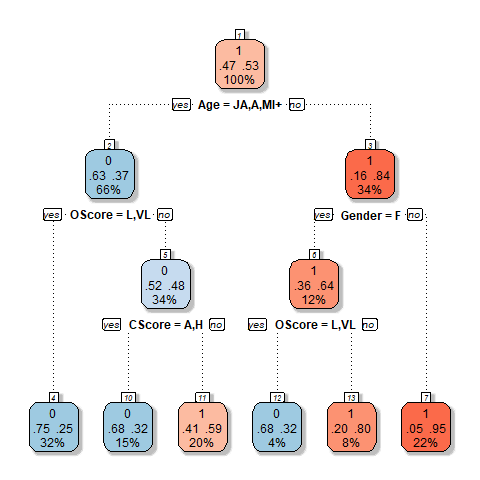
\includegraphics[height=8cm]{figuras/arvore_cannabis.png}}}%
    \caption{Visualização da árvore de decisão para a droga cannabis}
    \label{fig_DTCannabis}
\end{figure}

Realizados esses passos, aplicou-se o método de poda da árvore. A árvore podada acabou resultando na própria árvore original, indicando que o modelo anterior já é o mais parsimonioso que conseguimos obter para essa análise.


%\subsubsection{Comparação e Escolha do Modelo e Método}

%- comparar

%- escolher o melhor e executar resultados finais (acuracia, sensibilidade, ...)


% ----------------------------------------------------------
% 4.2 - Ecstasy
% ----------------------------------------------------------

\subsection{Ecstasy}

Na amostra coletada, tem-se que apenas 27,42\% dos indivíduos são usuários de Ecstasy. Este desbalanceamento tem efeito na sensibilidade do modelo, portanto, buscou-se corrigí-lo com técnicas de atribuição de pesos e penalidades.

\subsubsection{Regressão Logística}

As variáveis selecionadas foram: \textbf{Idade (Age), Gênero (Gender), Educação (Education) e Abertura (OScore)}. 

Observa-se na Tabela \ref{tabela_RegLogEcstasy} a matriz de confusão do modelo no conjunto de treino apenas com as variáveis selecionadas e o ponto de corte em 0,5. A acurácia do modelo foi relativamente alta, de 74,77\% , e a especificidade (93,71\%) também. Porém, a sensibilidade foi apenas 24,49\%, pois o banco de dados possui muito menos usuários do que não usuários e o modelo estimado acaba atribuindo baixas probabilidades aos usuários.

\begin{table}[H]
\centering
\begin{tabular}{cc|c|c|c}
\cline{3-4}
 & & \multicolumn{2}{c|}{Valor Verdadeiro} & \\ \cline{3-4}
 & & Positivo & Negativo & \\ \cline{1-4}
\multicolumn{1}{|c|}{\multirow{2}{*}{\rotatebox[origin=c]{90}{Valor Previsto}}} & \multicolumn{1}{c|}{\rotatebox[origin=c]{90}{ Positivo }} & \multicolumn{1}{c|}{107} & 73 & \\ \cline{2-4}
\multicolumn{1}{|c|}{} & \multicolumn{1}{c|}{\rotatebox[origin=c]{90}{ Negativo }} & \multicolumn{1}{c|}{330} & 1087 & \\ \cline{1-4}
\end{tabular}
\caption{Matriz de confusão da regressão logística no conjunto de treino para a droga ecstasy com ponto de corte em 0,5.}
\label{tabela_RegLogEcstasy}
\end{table}

Para buscar corrigir o desbalanceamento, executou-se a regressão logística com seleção de variáveis no conjunto de treino, mas adicionando peso \textbf{3} para usuários e \textbf{1} para não usuários. As variáveis selecionadas aumentaram, sendo incluídas \textbf{Conscienciosidade (CScore) e Socialização (AScore)}. Observamos na Tabela \ref{tabela_RegLogEcstasyWeightedTrain} que a especificidade reduziu para 78,88\%. Porém, a acurácia e a sensibilidade, que são as métricas de interesse, aumentaram para, respectivamente, 76,08\% e 68,65\%. 

Os coeficientes estimados pelo modelo podem ser visualizado na Tabela \ref{coef_reglog_ecstasy}.

\begin{table}[H]
\centering
\begin{tabular}{|l|r|}
\hline
Intercept                                                     & 0.0742 \\ \hline
Age25-34                                                      & -0.6736 \\ \hline
Age35-44                                                      & -1.7943 \\ \hline    
Age45+                                                        & -2.3933 \\ \hline
GenderMale                                                    & 0.6453  \\ \hline
EducationLeft school                                          & 0.4383  \\ \hline
EducationProfessional certificate/ diploma                    & 0.3875  \\ \hline
EducationSome college or university, no certificate or degree & 0.4939  \\ \hline
EducationUniversity degree                                    & 0.0995  \\ \hline
CScoreHigh                                                    & -0.2756 \\ \hline
CScoreLow                                                     & 0.2892  \\ \hline
CScoreVeryLow                                                 & 0.2665  \\ \hline
AScoreHigh                                                    & -0.5383 \\ \hline
AScoreLow                                                     & 0.2423  \\ \hline
AScoreVeryLow                                                 & 0.4482  \\ \hline
OScoreHigh                                                    & 0.6693  \\ \hline
OScoreLow                                                     & -0.6911 \\ \hline
OScoreVeryLow                                                 & -0.5869 \\ \hline
\end{tabular}
\caption{Coeficientes da Regressão Logística para o Ecstasy}
\label{coef_reglog_ecstasy}
\end{table}

\vspace{2cm}

\begin{table}[H]
\centering
\begin{tabular}{cc|c|c|c}
\cline{3-4}
 & & \multicolumn{2}{c|}{Valor Verdadeiro} & \\ \cline{3-4}
 & & Positivo & Negativo & \\ \cline{1-4}
\multicolumn{1}{|c|}{\multirow{2}{*}{\rotatebox[origin=c]{90}{Valor Previsto}}} & \multicolumn{1}{c|}{\rotatebox[origin=c]{90}{ Positivo }} & \multicolumn{1}{c|}{300} & 245 & \\ \cline{2-4}
\multicolumn{1}{|c|}{} & \multicolumn{1}{c|}{\rotatebox[origin=c]{90}{ Negativo }} & \multicolumn{1}{c|}{137} & 915 & \\ \cline{1-4}
\end{tabular}
\caption{Matriz de confusão do conjunto de treino da regressão logística com pesos para a droga ecstasy com ponto de corte em 0,5.}
\label{tabela_RegLogEcstasyWeightedTrain}
\end{table}

\begin{figure}[H]
    \centering
    \textbf{Probabilidade predita e classe verdadeira}\par\medskip
    \subfloat{{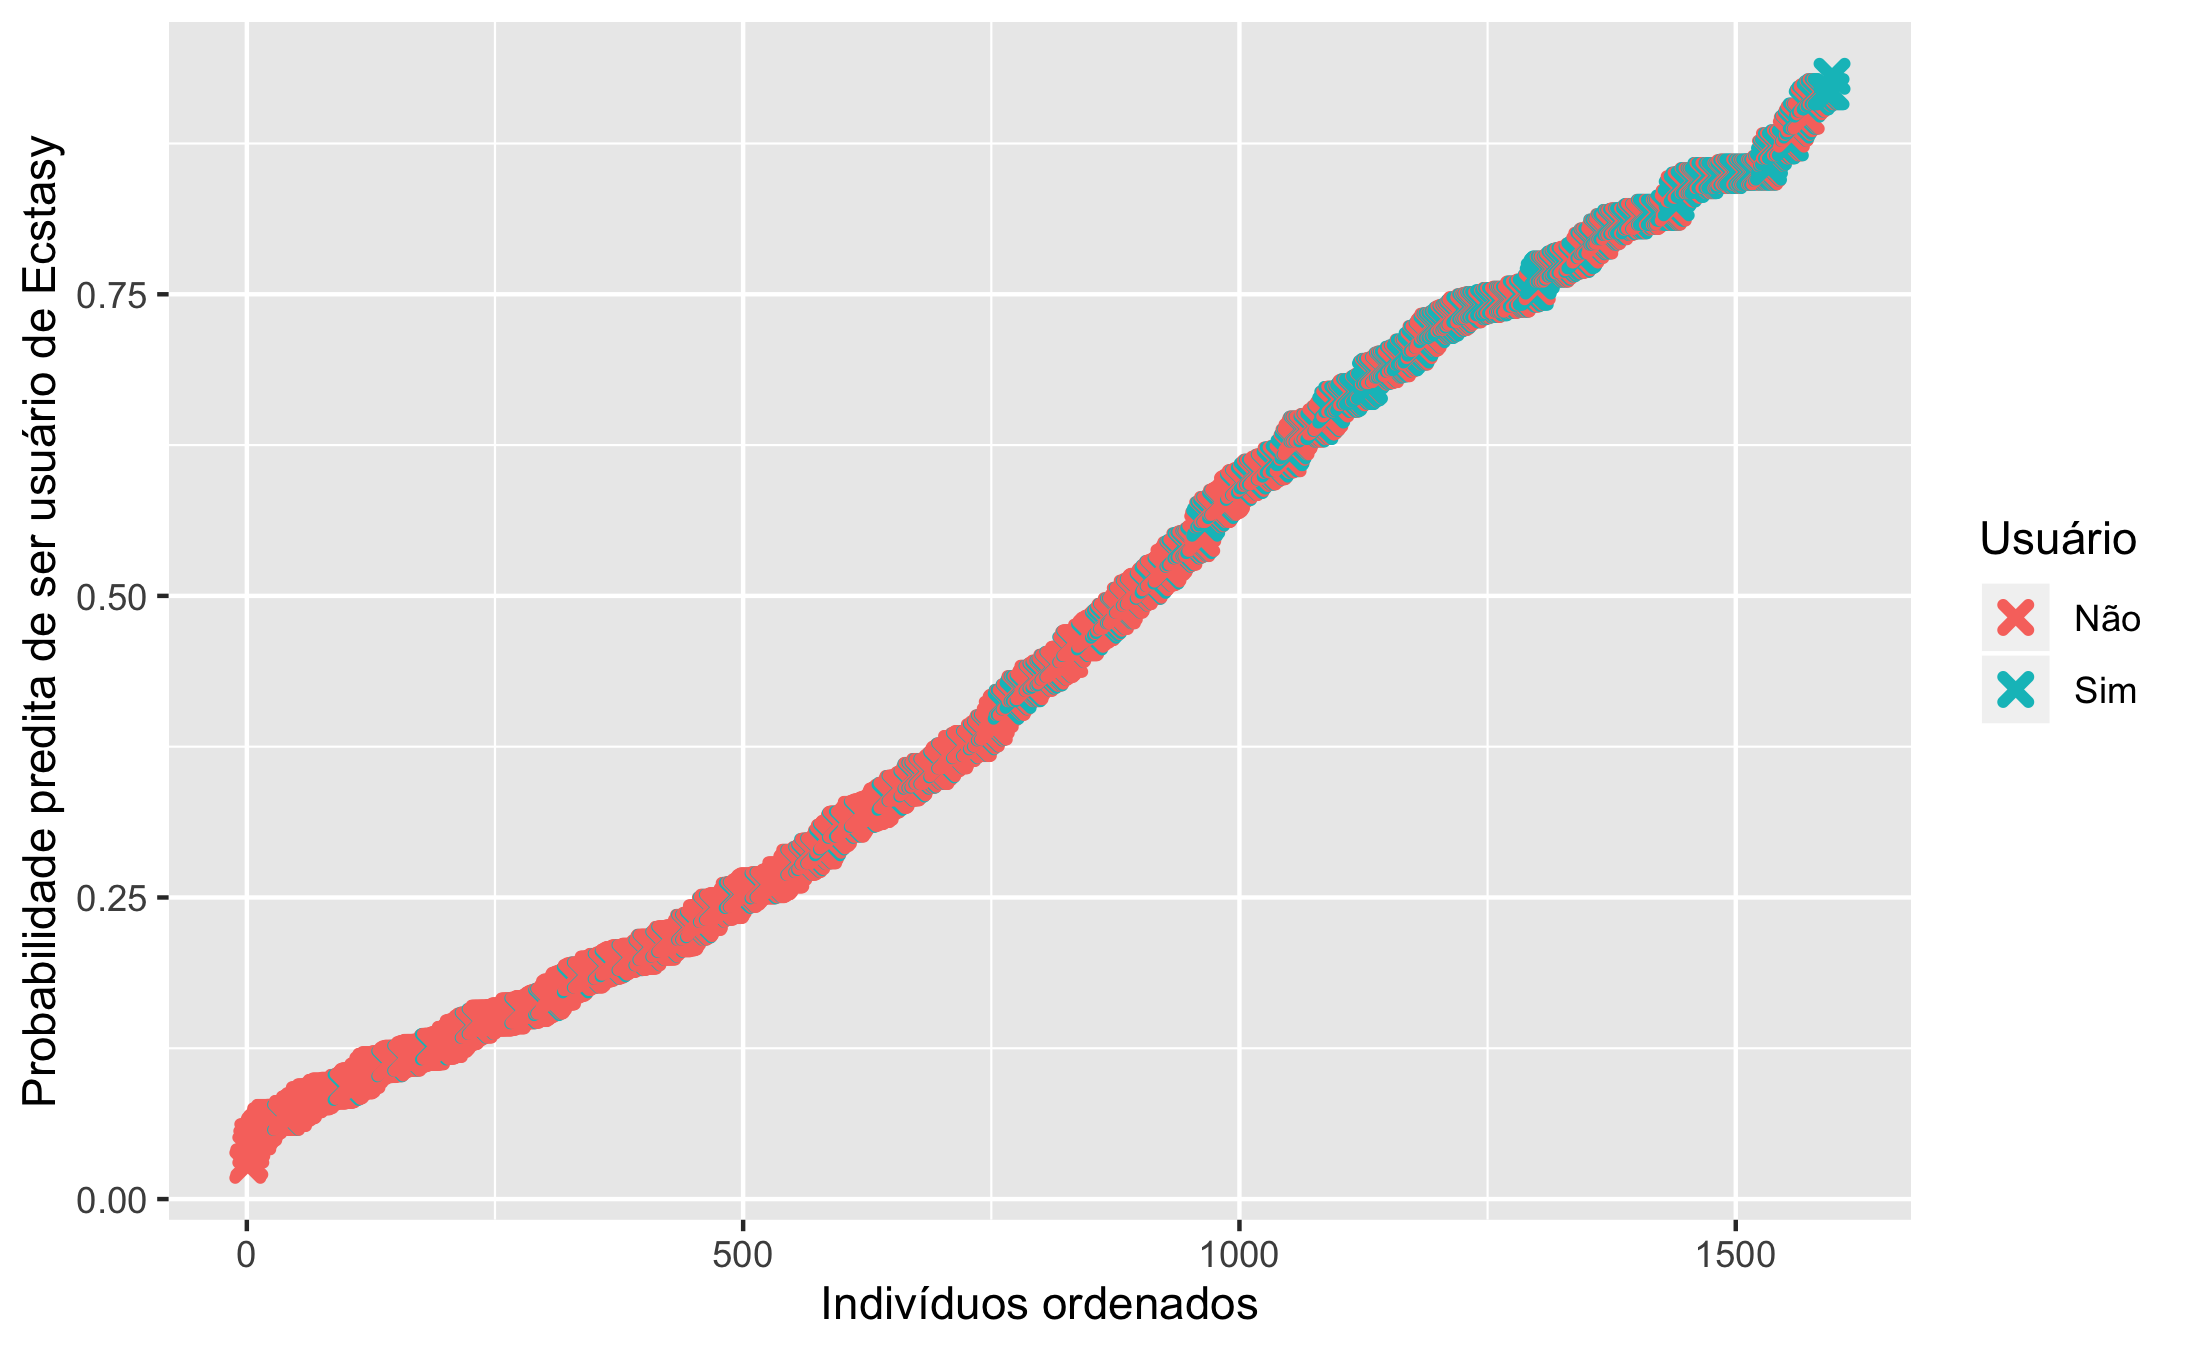
\includegraphics[width=13cm]{figuras/LogRegEcstasyWeighted.png}}}%
    \caption{Gráfico da probabilidade predita e respectiva classe das observações dos usuários de ecstasy}
    \label{fig_LogRegEcstasyWeighted}
\end{figure}

Observa-se no gráfico da Figura \ref{fig_LogRegEcstasyWeighted} que o ponto de corte em torno de 0,5 é adequado e optou-se por mantê-lo. 

Utilizando modelo ajustado com pesos e ponto de corte em 0,5 no conjunto de teste, pode-se observar que os valores de acurácia, sensibilidade e especificidade ficaram próximos, tendo a sensibilidade reduzido para 65,79\% e a acurácia e especificidade aumentado para 77,14\% e 81,37\%, respectivamente, como observado nas Tabelas \ref{tabela_RegLogEcstasyWeighted} e \ref{resultadosreglog_ecstasy}. 

\begin{table}[H]
\centering
\begin{tabular}{cc|c|c|c}
\cline{3-4}
 & & \multicolumn{2}{c|}{Valor Verdadeiro} & \\ \cline{3-4}
 & & Positivo & Negativo & \\ \cline{1-4}
\multicolumn{1}{|c|}{\multirow{2}{*}{\rotatebox[origin=c]{90}{Valor Previsto}}} & \multicolumn{1}{c|}{\rotatebox[origin=c]{90}{ Positivo }} & \multicolumn{1}{c|}{50} & 38 & \\ \cline{2-4}
\multicolumn{1}{|c|}{} & \multicolumn{1}{c|}{\rotatebox[origin=c]{90}{ Negativo }} & \multicolumn{1}{c|}{26} & 166 & \\ \cline{1-4}
\end{tabular}
\caption{Matriz de confusão do conjunto de teste da regressão logística com pesos para a droga ecstasy com ponto de corte em 0,5.}
\label{tabela_RegLogEcstasyWeighted}
\end{table}

\begin{table}[H]
\centering
\begin{tabular}{||c|c|c|c||}
\hline
Conjunto & Acurácia & Sensibilidade & Especificidade \\ \hline
Treino (corte 0,5) & 74,77\% & 24,49\% & 93,71\% \\ \hline
Treino com pesos (corte 0,5) & 76,08\% & 68,65\% & 78,88\% \\ \hline
Teste com pesos (corte 0,5) & 77,14\% & 65,79\% & 81,37\% \\ \hline
\end{tabular}
\caption{Métricas de performance da regressão logística para a droga ecstasy.}
\label{resultadosreglog_ecstasy}
\end{table}


Através dos valores \emph{odds ratio} das variáveis, sugere-se que o \emph{score} alto na característica Abertura (O) aumenta a chance de uma pessoa ser usuária de Ecstasy em 1,95 vezes, o \emph{score} muito baixo em Socialização (A) aumenta em 1,57 vezes, e o \emph{score} muito baixo em Conscienciosidade (C) aumenta em 1,31 vezes, quando comparados aos indivíduos com \emph{scores} medianos. Ainda, homens têm 1,91 vezes mais chance de serem usuários do que mulheres.


\subsubsection{Árvore de Decisão}

Para a droga ecstasy, obteve-se um modelo com as seguintes variáveis: \textbf{Idade (Age), Conscienciosidade (CScore), Gênero (Gender), Abertura (OScore), Extorversão (Escore)}. Apesar da acurácia do ajuste ser relativamente alta, em cerca de 77\%, a sensibilidade do ajuste fica consideravelmente baixa, na faixa dos 40\%. Os resultados compilados estão na Tabela \ref{resultadosdt_ecstasy} e a matriz de confusão para o conjunto de teste pode ser observada em \ref{matrizconfusaodt_ecstasy}. A visualização da árvore produzida pode ser observada na Figura \ref{fig_DTEcstasy}.
\vspace{0.5cm}

\begin{table}[H]
\centering
\begin{tabular}{||c|c|c|c||}
\hline
Conjunto & Acurácia & Sensibilidade & Especificidade \\ \hline
Treino & 76,58\% & 43,71\% & 88,97\% \\ \hline
Teste & 77,14\% & 40,79\% & 90,69\% \\ \hline
\end{tabular}
\caption{Métricas de performance da árvore de decisão para a droga ecstasy.}
\label{resultadosdt_ecstasy}
\end{table}

\vspace{1cm}

\begin{table}[H]
\centering
\begin{tabular}{cc|c|c|c}
\cline{3-4}
 & & \multicolumn{2}{c|}{Valor Verdadeiro} & \\ \cline{3-4}
 & & Positivo & Negativo & \\ \cline{1-4}
\multicolumn{1}{|c|}{\multirow{2}{*}{\rotatebox[origin=c]{90}{Valor Previsto}}} & \multicolumn{1}{c|}{\rotatebox[origin=c]{90}{ Positivo }} & \multicolumn{1}{c|}{31} & 19 & \\ \cline{2-4}
\multicolumn{1}{|c|}{} & \multicolumn{1}{c|}{\rotatebox[origin=c]{90}{ Negativo }} & \multicolumn{1}{c|}{45} & 185 & \\ \cline{1-4}
\end{tabular}
\caption{Tabela de confusão do conjunto de teste da árvore de decisão para a droga ecstasy.}
\label{matrizconfusaodt_ecstasy}
\end{table}

\begin{figure}[H]
    \centering
    \textbf{Árvore de Decisão - Ecstasy}\par\medskip
    \subfloat{{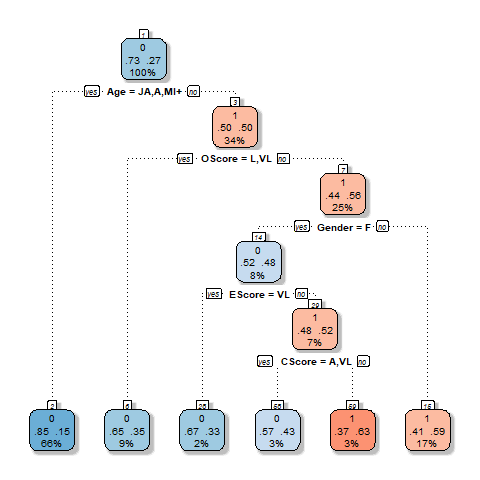
\includegraphics[height=10cm]{figuras/arvore_ecstasy.png}}}%
    \caption{Visualização da árvore de decisão para a droga ecstasy}
    \label{fig_DTEcstasy}
\end{figure}

\vspace{0.5cm}

Devido à baixa sensibilidade obtida no ajuste, decidiu-se refazer a análise utilizando uma matriz de perda que focasse mais na predição correta dos usuários - ou seja, o erro de classificar usuários como não usuários foi considerado duas vezes pior que cometer o erro o inverso. Dessa vez, o modelo obtido continha as variáveis \textbf{Idade (Age), Gênero (Gender), Abertura (OScore)}. A acurácia do ajuste baixou apenas 3\%, permanecendo acima dos 70\%, enquanto a sensibilidade subiu em quase 30\% - e esse resultado é exatamente o que se desejava obter aplicando a penalização sobre os erros. A Tabela \ref{resultadosdt_loss_ecstasy} apresenta os resultados obtidos, enquanto a matriz de confusão está na Tabela \ref{matrizconfusaodt_loss_ecstasy}. A visualização da nova árvore pode ser vista na Figura \ref{fig_DTEcstasy_loss}.

\vspace{1cm}

\begin{table}[H]
\centering
\begin{tabular}{||c|c|c|c||}
\hline
Conjunto & Acurácia & Sensibilidade & Especificidade \\ \hline
Treino & 73,32\% & 76,20\% & 72,24\% \\ \hline
Teste & 74,64\% & 69,34\% & 76,47\% \\ \hline
\end{tabular}
\caption{Métricas de performance da árvore de decisão com função perda modificada para a droga ecstasy.}
\label{resultadosdt_loss_ecstasy}
\end{table}

\begin{table}[H]
\centering
\begin{tabular}{cc|c|c|c}
\cline{3-4}
 & & \multicolumn{2}{c|}{Valor Verdadeiro} & \\ \cline{3-4}
 & & Positivo & Negativo & \\ \cline{1-4}
\multicolumn{1}{|c|}{\multirow{2}{*}{\rotatebox[origin=c]{90}{Valor Previsto}}} & \multicolumn{1}{c|}{\rotatebox[origin=c]{90}{ Positivo }} & \multicolumn{1}{c|}{53} & 48 & \\ \cline{2-4}
\multicolumn{1}{|c|}{} & \multicolumn{1}{c|}{\rotatebox[origin=c]{90}{ Negativo }} & \multicolumn{1}{c|}{23} & 156 & \\ \cline{1-4}
\end{tabular}
\caption{Tabela de confusão do conjunto de teste da árvore de decisão com função perda modificada para a droga ecstasy.}
\label{matrizconfusaodt_loss_ecstasy}
\end{table}

\begin{figure}[H]
    \centering
    \textbf{Árvore de Decisão Penalizada - Ecstasy}\par\medskip
    \subfloat{{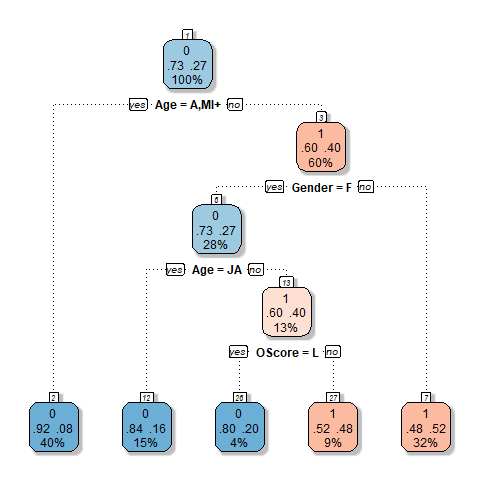
\includegraphics[height=8cm]{figuras/arvore_ecstasy_pesada.png}}}%
    \caption{Visualização da árvore de decisão com função perda modificada para a droga ecstasy}
    \label{fig_DTEcstasy_loss}
\end{figure}

Por fim, aplicou-se o método de poda sobre a árvore com função perda modificada. A árvore podada obtida corresponde a um modelo apenas com as variáveis \textbf{Idade (Age), Gênero (Gender)}. Apesar da especificidade da árvore podada aumentar cerca de 5\%, a acurácia aumenta menos de 1\% e a sensibilidade do ajuste baixa em torno de 15\%, como pode ser visto na Tabela \ref{resultados_ecstasy_podada}. Como as últimas métricas são consideradas mais essenciais para a análise, optou-se por não adotar a árvore podada e permanecer apenas com a árvore penalizada. 

\begin{table}[H]
\centering
\begin{tabular}{||c|c|c|c||}
\hline
Conjunto & Acurácia & Sensibilidade & Especificidade \\ \hline
Treino & 73,76\% & 60,41\% & 78,79\% \\ \hline
Teste & 75,00\% & 56,58\% & 81,86\% \\ \hline
\end{tabular}
\caption{Métricas de performance da árvore de decisão para a droga ecstasy.}
\label{resultados_ecstasy_podada}
\end{table}

% ----------------------------------------------------------
% 4.3 - Álcool
% ----------------------------------------------------------

\subsection{Álcool}

Foi observado que a amostra utilizada para avaliar se um indivíduo é ou não usuário de álcool é exageradamente desigual: apenas 7\% dos indivíduos da amostra não são usuários. Isso torna a predição do modelo muito difícil, de tal forma que nenhum dos modelos estimados possui boas propriedades. 

\subsubsection{Regressão Logística}

Na regressão logística, mesmo atribuindo um peso oito vezes maior aos não usuários, não é possível ter uma acurácia aceitável, de forma que classificar sempre o indivíduo como usuário tem melhores resultados do que executar o modelo.

\begin{table}[H]
\centering
\begin{tabular}{||c|c|c|c||}
\hline
Conjunto & Acurácia & Sensibilidade & Especificidade \\ \hline
Treino & 61,09\% & 62,60\% & 60,97\% \\ \hline
Teste & 56,58\% & 75,00\% & 55,17\% \\ \hline
\end{tabular}
\caption{Métricas de performance da regressão logística para a droga álcool.}
\label{resultados_reglogalcool}
\end{table}

Os coeficientes estimados pelo modelo podem ser visualizado na Tabela \ref{coef_reglog_alcohol}.

\begin{table}[H]
\centering
\begin{tabular}{|l|r|}
\hline
Intercept                                                     & 0.9699 \\ \hline

Age25-34                                                      & -0.2805 \\ \hline
Age35-44                                                      & -0.6758 \\ \hline
Age45+                                                        & -0.9388 \\ \hline
GenderMale                                                    & -0.2370  \\ \hline
EducationLeft school                                          & -0.6666 \\ \hline
EducationProfessional certificate/ diploma                    & -0.5805 \\ \hline
EducationSome college or university, no certificate or degree & -0.3705\\ \hline
EducationUniversity degree                                    & -0.2764  \\ \hline
NScoreHigh                                                    & 0.2320\\ \hline
NScoreLow                                                     & 0.2912  \\ \hline
NScoreVeryLow                                                 & 0.3909 \\ \hline
CScoreHigh                                                    & 0.6059 \\ \hline
CScoreLow                                                     & 0.3635  \\ \hline
CScoreVeryLow                                                 & 0.5160  \\ \hline

AScoreHigh                                                    & -0.4261 \\ \hline
AScoreLow                                                     & 0.1961  \\ \hline
AScoreVeryLow                                                 & 0.2040  \\ \hline

EScoreHigh                                                    & 13.5985  \\ \hline
EScoreLow                                                     & -0.2406 \\ \hline
EScoreVeryLow                                                 & -0.2219 \\ \hline
\end{tabular}
\caption{Coeficientes da Regressão Logística para o Álcool}
\label{coef_reglog_alcohol}
\end{table}


\subsubsection{Árvore de Decisão}

Para o álcool, houveram dificuldades de ajustar uma árvore de decisão: devido a altíssima proporção de usuários de álcool na base, não foi possível gerar modelos. O algoritmo não consegue obter nenhuma partição que diminua a impureza, então ele retorna apenas uma raiz. A única maneira de se gerar um modelo de árvore de decisão nesse caso é forçando a criação de uma árvore sobreajustada que utiliza todos os atributos disponíveis. Apesar das métricas do ajuste forçado serem incrivelmente altas, como é possível observar na Tabela \ref{resultadosdt_alcool}, isso deve-se apenas ao viés inerente da base. Analisando-se a Figura \ref{fig_DTAlcohol}, nota-se com clareza que o modelo gerado é de péssima qualidade e que ele falha em resolver o problema de classificação.

\begin{table}[H]
\centering
\begin{tabular}{||c|c|c|c||}
\hline
Conjunto & Acurácia & Sensibilidade & Especificidade \\ \hline
Treino & 97,30\% & 99,80\% & 65,22\% \\ \hline
Teste & 85,76\% & 91,19\% & 15,00\% \\ \hline
\end{tabular}
\caption{Métricas de performance da árvore de decisão para a droga álcool.}
\label{resultadosdt_alcool}
\end{table}

\begin{figure}[H]
    \centering
    \textbf{Árvore de Decisão - Álcool}\par\medskip
    \subfloat{{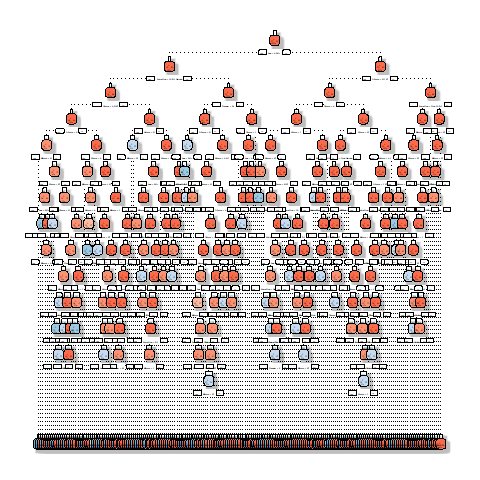
\includegraphics[width=13cm]{figuras/arvore_alcohol.png}}}%
    \caption{Visualização da árvore de decisão para a droga álcool}
    \label{fig_DTAlcohol}
\end{figure}

% ----------------------------------------------------------
% 4.4 - Grupo de Drogas Estimulantes
% ----------------------------------------------------------

\subsection{Grupo de Drogas Estimulantes}

A distribuição de usuários e não usuários de drogas estimulantes é de 67,5\% usuários e 32,5\% não usuários, o que nos leva a utilizar pesos e penalidades para buscar melhores resultados. 

\subsubsection{Regressão Logística}

As variáveis selecionadas foram: \textbf{Idade (Age), Gênero (Gender), Educação (Education), Abertura (OScore), Conscienciosidade (CScore) e Socialização (AScore)}. 

Ajustando o modelo no conjunto de treino com as variáveis selecionadas e o ponto de corte em 0,5, obteve-se 70,93\% de acurácia, 93,22\% de especificidade, mas apenas 24,51\% de sensibilidade, como observado nas Tabelas \ref{tabela_RegLogEstimulantesTreino} e \ref{resultadosreglog_estimulantes}. Similarmente ao método empregado para a droga ecstasy, atribuiu-se um peso maior aos usuários de drogas estimulantes para buscar melhores resultados na métrica sensibilidade. Para seguir a proporção da amostra, utilizou-se peso \textbf{2} para usuários e \textbf{1} para não usuários. As variáveis selecionadas se mantiveram as mesmas e foi possível aumentar a acurácia e a sensibilidade para 72,81\% e 52,90\%, respectivamente, como apresentado nas Tabelas \ref{tabela_RegLogEstimulantesTreinoPesos} e \ref{resultadosreglog_estimulantes}.


\begin{table}[H]
\centering
\begin{tabular}{cc|c|c|c}
\cline{3-4}
 & & \multicolumn{2}{c|}{Valor Verdadeiro} & \\ \cline{3-4}
 & & Positivo & Negativo & \\ \cline{1-4}
\multicolumn{1}{|c|}{\multirow{2}{*}{\rotatebox[origin=c]{90}{Valor Previsto}}} & \multicolumn{1}{c|}{\rotatebox[origin=c]{90}{ Positivo }} & \multicolumn{1}{c|}{127} & 73 & \\ \cline{2-4}
\multicolumn{1}{|c|}{} & \multicolumn{1}{c|}{\rotatebox[origin=c]{90}{ Negativo }} & \multicolumn{1}{c|}{391} & 1005 & \\ \cline{1-4}
\end{tabular}
\caption{Matriz de confusão da regressão logística no conjunto de treino para o grupo de drogas estimulantes.}
\label{tabela_RegLogEstimulantesTreino}
\end{table}

\begin{table}[H]
\centering
\begin{tabular}{cc|c|c|c}
\cline{3-4}
 & & \multicolumn{2}{c|}{Valor Verdadeiro} & \\ \cline{3-4}
 & & Positivo & Negativo & \\ \cline{1-4}
\multicolumn{1}{|c|}{\multirow{2}{*}{\rotatebox[origin=c]{90}{Valor Previsto}}} & \multicolumn{1}{c|}{\rotatebox[origin=c]{90}{ Positivo }} & \multicolumn{1}{c|}{274} & 190 & \\ \cline{2-4}
\multicolumn{1}{|c|}{} & \multicolumn{1}{c|}{\rotatebox[origin=c]{90}{ Negativo }} & \multicolumn{1}{c|}{244} & 888 & \\ \cline{1-4}
\end{tabular}
\caption{Tabela de confusão da regressão logística com pesos no conjunto de treino para o grupo de drogas estimulantes.}
\label{tabela_RegLogEstimulantesTreinoPesos}
\end{table}

Ainda, o gráfico apresentado na Figura \ref{fig_LogRegEstimulanteWeighted} sugere que é possível aumentar a métrica de interesse reduzindo o ponto de corte. Classificando como usuários os indivíduos com probabilidade predita maior ou igual a 0,35, obteve-se um aumento na sensibilidade para 59,27\%, sem comprometer a acurácia, que ficou muito próxima (72,74\%) e compromentendo a especificidade, que reduziu para 79,22\%.


Os coeficientes estimados pelo modelo podem ser visualizado na Tabela \ref{coef_reglog_stimulants}.

\begin{table}[H]
\centering
\begin{tabular}{|l|r|}
\hline
Intercept                                                     & -0.6014 \\ \hline

Age25-34                                                      & -0.2366 \\ \hline
Age35-44                                                      & -1.0288 \\ \hline
Age45+                                                        & -1.6973 \\ \hline
GenderMale                                                    & 0.5969  \\ \hline
EducationLeft school                                          & 0.4797  \\ \hline
EducationProfessional certificate/ diploma                    & 0.3919  \\ \hline
EducationSome college or university, no certificate or degree & 0.5741 \\ \hline
EducationUniversity degree                                    & 0.0581  \\ \hline

CScoreHigh                                                    & 0.335 \\ \hline
CScoreLow                                                     & 0.3863  \\ \hline
CScoreVeryLow                                                 & 0.958  \\ \hline

AScoreHigh                                                    & -0.3841 \\ \hline
AScoreLow                                                     & 0.3295  \\ \hline
AScoreVeryLow                                                 & 0.9352  \\ \hline

OScoreHigh                                                    & 0.5459  \\ \hline
OScoreLow                                                     & -0.6141 \\ \hline
OScoreVeryLow                                                 & -0.6744 \\ \hline
\end{tabular}
\caption{Coeficientes da Regressão Logística para o grupo de Drogas Estimulantes}
\label{coef_reglog_stimulants}
\end{table}

\begin{figure}[H]
    \centering
    \textbf{Probabilidade predita e classe verdadeira}\par\medskip
    \subfloat{{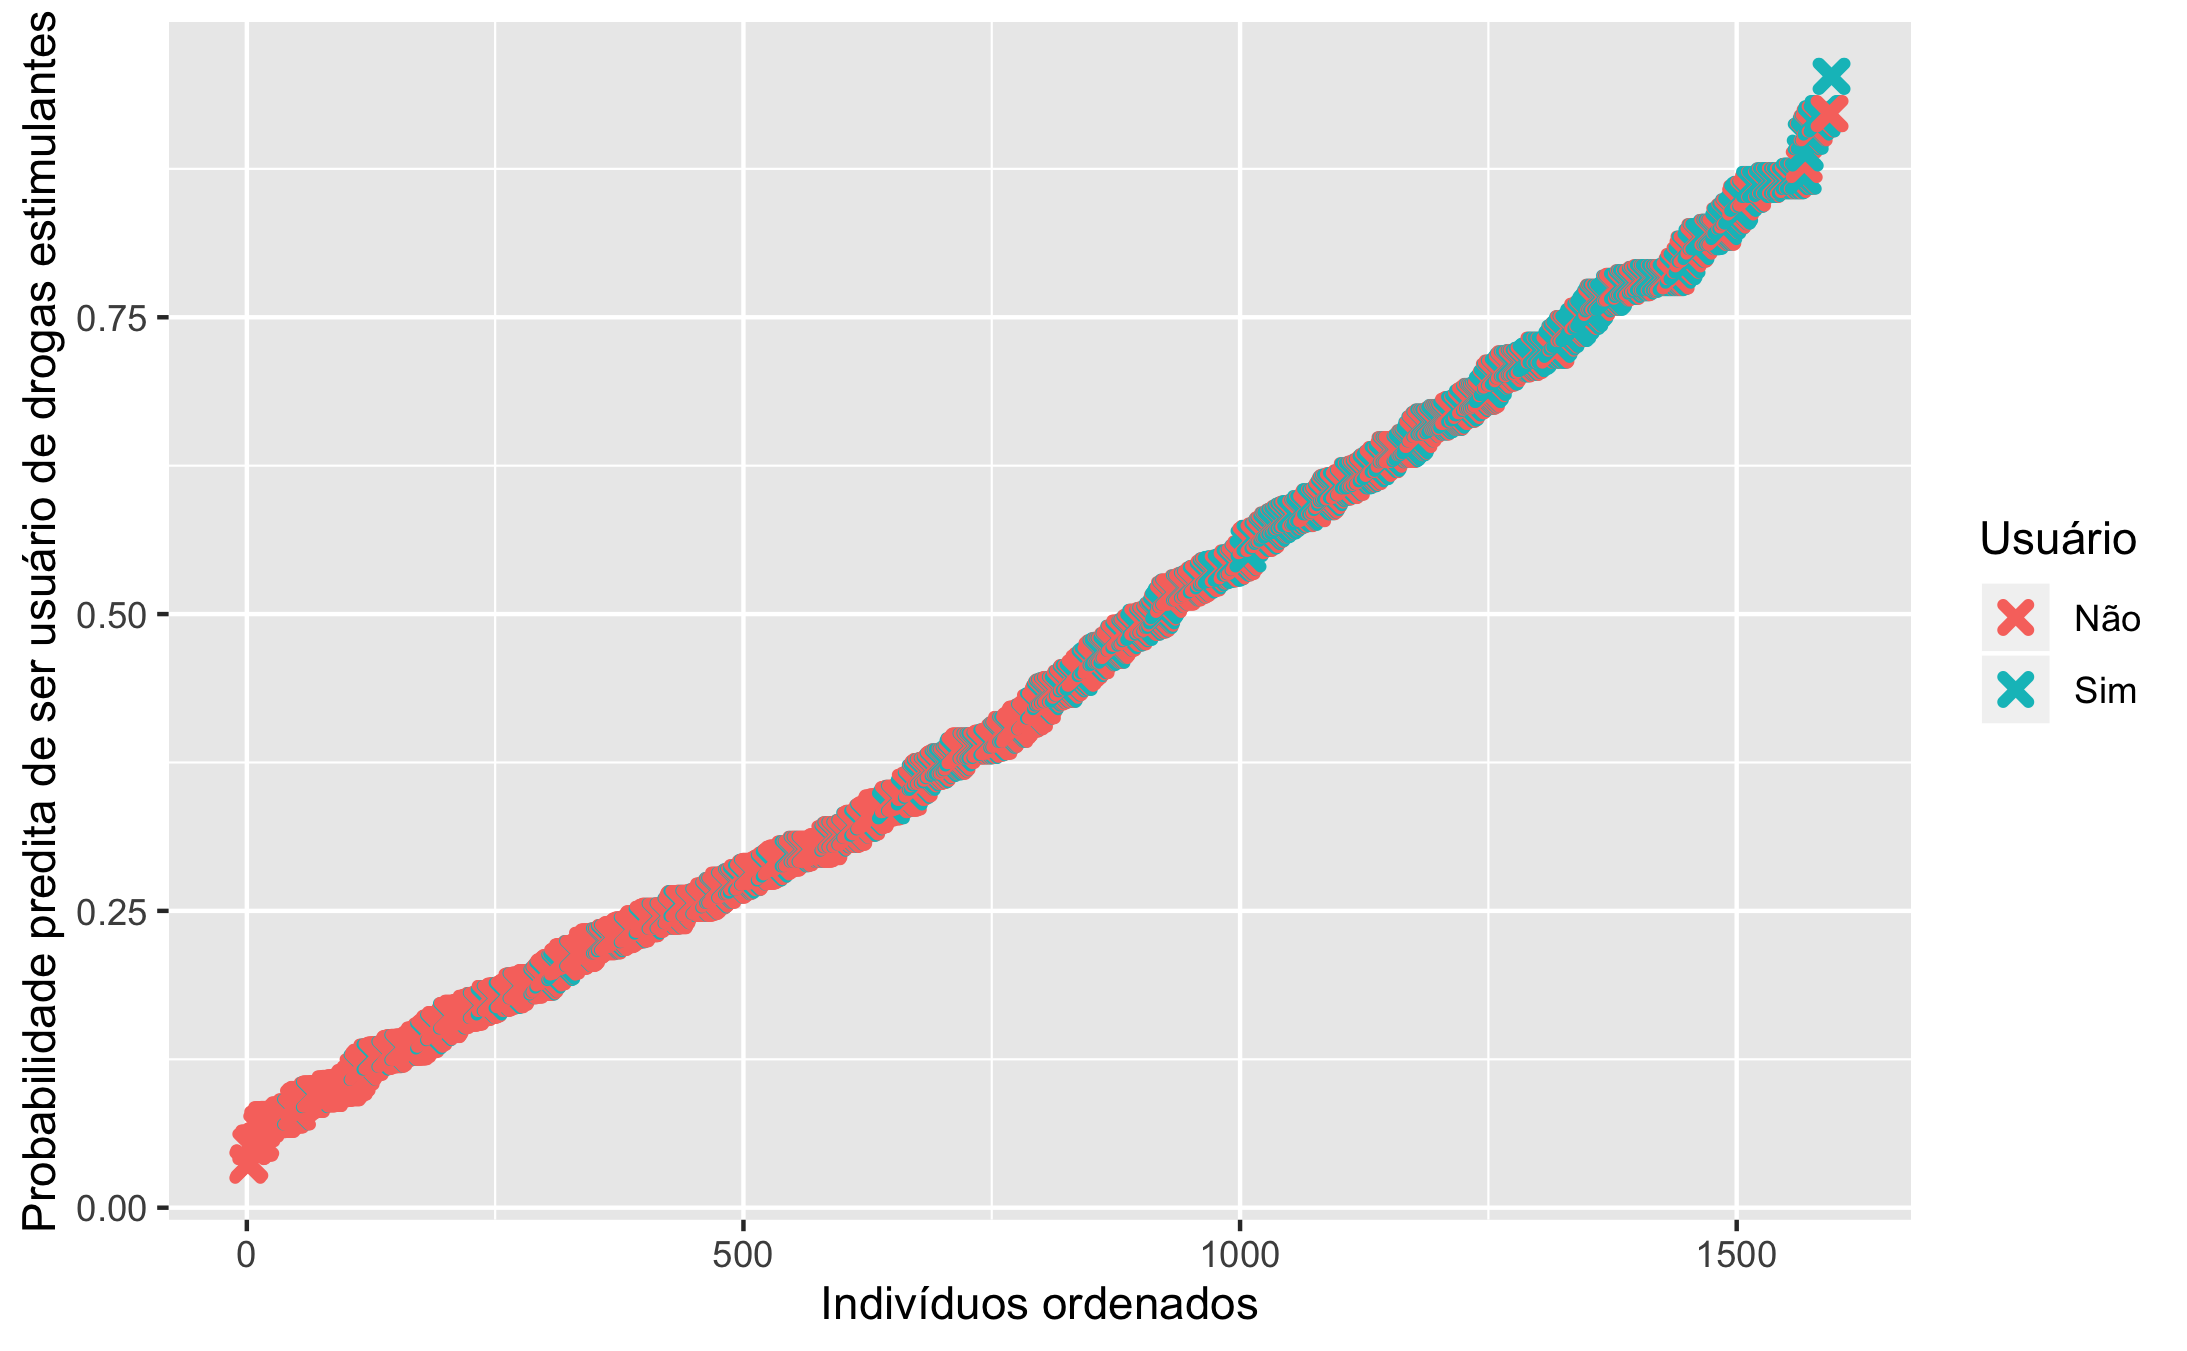
\includegraphics[width=13cm]{figuras/LogRegEstimulantes.png}}}%
    \caption{Gráfico da probabilidade predita e respectiva classe das observações dos usuários de drogas estimulantes}
    \label{fig_LogRegEstimulanteWeighted}
\end{figure}

\begin{table}[H]
\centering
\begin{tabular}{cc|c|c|c}
\cline{3-4}
 & & \multicolumn{2}{c|}{Valor Verdadeiro} & \\ \cline{3-4}
 & & Positivo & Negativo & \\ \cline{1-4}
\multicolumn{1}{|c|}{\multirow{2}{*}{\rotatebox[origin=c]{90}{Valor Previsto}}} & \multicolumn{1}{c|}{\rotatebox[origin=c]{90}{ Positivo }} & \multicolumn{1}{c|}{307} & 224 & \\ \cline{2-4}
\multicolumn{1}{|c|}{} & \multicolumn{1}{c|}{\rotatebox[origin=c]{90}{ Negativo }} & \multicolumn{1}{c|}{211} & 854 & \\ \cline{1-4}
\end{tabular}
\caption{Tabela de confusão da regressão logística com pesos no conjunto de treino e ponto de corte em 0,35 para o grupo de drogas estimulantes.}
\label{tabela_RegLogEstimulantesTreinoPesos035}
\end{table}

A Tabela \ref{tabela_RegLogEstimulantesTeste} apresenta a matriz de confusão com os resultados da aplicação do modelo estimado no conjunto de teste, com peso 2 atribuído a usuários de drogas estimulantes e 1 para não usuários e ponto de corte em 0,35. Observa-se que acurácia ficou em 70,82\%, a sensibilidade aumentou para 63,74\% e a especificidade reduziu para 74,21\%. Considerou-se um bom ajuste, dado que as métricas de interesse foram satisfatórias.

\begin{table}[H]
\centering
\begin{tabular}{cc|c|c|c}
\cline{3-4}
 & & \multicolumn{2}{c|}{Valor Verdadeiro} & \\ \cline{3-4}
 & & Positivo & Negativo & \\ \cline{1-4}
\multicolumn{1}{|c|}{\multirow{2}{*}{\rotatebox[origin=c]{90}{Valor Previsto}}} & \multicolumn{1}{c|}{\rotatebox[origin=c]{90}{ Positivo }} & \multicolumn{1}{c|}{58} & 49 & \\ \cline{2-4}
\multicolumn{1}{|c|}{} & \multicolumn{1}{c|}{\rotatebox[origin=c]{90}{ Negativo }} & \multicolumn{1}{c|}{33} & 141 & \\ \cline{1-4}
\end{tabular}
\caption{Tabela de confusão da regressão logística com pesos no conjunto de teste e ponto de corte em 0,35 para o grupo de drogas estimulantes.}
\label{tabela_RegLogEstimulantesTeste}
\end{table}


Percebe-se, através da avaliação dos valores de \emph{odds ratio} das variáveis, que indivíduos com \emph{scores} de Conscienciosidade (C) e Socialização (A) muito baixos possuem 2,61 e 2,55 vezes, respectivamente, mais chance de serem usuários de drogas estimulantes quando comparados a indivíduos com \emph{score} mediano. Ainda, pessoas com mais de 45 anos de idade têm 82\% menos chance de serem usuários do que os jovens entre 18 e 24 anos, e homens têm 1,82 vezes mais possibilidade de serem usuários do que mulheres.


\begin{table}[H]
\centering
\begin{tabular}{||c|c|c|c||}
\hline
Conjunto & Acurácia & Sensibilidade & Especificidade \\ \hline
Treino (corte 0,5) & 70,93\% & 24,51\% & 93,22\% \\ \hline
Treino com pesos (corte 0,5) & 72,81\% & 52,90\% & 82,37\% \\ \hline
Treino com pesos (corte 0,35) & 72,74\% & 59,27\% & 79,22\% \\ \hline
Teste com pesos (corte 0,35) & 70,82\% & 63,74\% & 74,21\% \\ \hline
\end{tabular}
\caption{Métricas de performance da regressão logística para a drogas estimulantes.}
\label{resultadosreglog_estimulantes}
\end{table}


\subsubsection{Árvore de Decisão}

Para o conjunto de drogas estimulantes, obteve-se um modelo com as variáveis \textbf{Idade (Age), Socialização (AScore), Educação (Education), Gênero (Gender), Neuroticismo (NScore), Abertura (OScore)}. Assim como no caso do ecstasy, a acurácia foi consideravelmente alta, na casa dos 70\%, mas a sensibilidade do ajuste não ultrapassa os 40\%, tal como pode ser visto na Tabela \ref{resultadosdt_stimulating}. A matriz de confusão para o conjunto de teste pode ser observada na Tabela \ref{matrizconfusaodt_stimulating}, enquanto a visualização da árvore produzida encontra-se na Figura \ref{fig_DTStimulating}.

\begin{table}[H]
\centering
\begin{tabular}{||c|c|c|c||}
\hline
Conjunto & Acurácia & Sensibilidade & Especificidade \\ \hline
Treino & 74,87\% & 40,15\% & 91,56\% \\ \hline
Teste & 71,53\% & 35,16\% & 88,95\% \\ \hline
\end{tabular}
\caption{Métricas de performance da árvore de decisão para o grupo de drogas estimulantes.}
\label{resultadosdt_stimulating}
\end{table}
\vspace{-0.5cm}
\begin{table}[H]
\centering
\begin{tabular}{cc|c|c|c}
\cline{3-4}
 & & \multicolumn{2}{c|}{Valor Verdadeiro} & \\ \cline{3-4}
 & & Positivo & Negativo & \\ \cline{1-4}
\multicolumn{1}{|c|}{\multirow{2}{*}{\rotatebox[origin=c]{90}{Valor Previsto}}} & \multicolumn{1}{c|}{\rotatebox[origin=c]{90}{ Positivo }} & \multicolumn{1}{c|}{32} & 21 & \\ \cline{2-4}
\multicolumn{1}{|c|}{} & \multicolumn{1}{c|}{\rotatebox[origin=c]{90}{ Negativo }} & \multicolumn{1}{c|}{59} & 169 & \\ \cline{1-4}
\end{tabular}
\caption{Tabela de confusão do conjunto de teste da árvore de decisão para o grupo de drogas estimulantes.}
\label{matrizconfusaodt_stimulating}
\end{table}

\begin{figure}[H]
    \centering
    \textbf{Árvore de Decisão - Drogas Estimulantes}\par\medskip
    \subfloat{{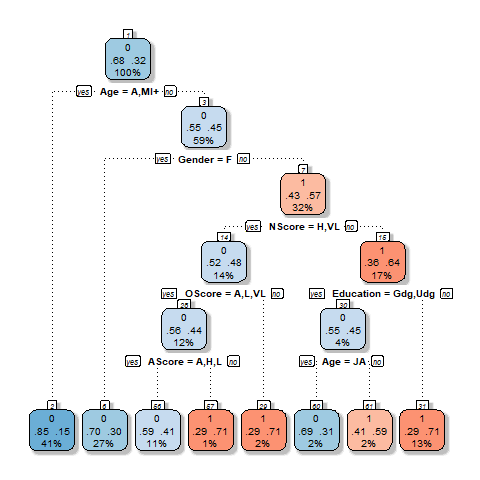
\includegraphics[height=7.5cm]{figuras/arvore_stimulating.png}}}%
    \caption{Visualização da árvore de decisão para o grupo de drogas estimulantes}
    \label{fig_DTStimulating}
\end{figure}

Seguindo as mesmas etapas realizadas para o ecastasy, a análise foi refeita considerando o erro de classificar usuários como não usuários como sendo duas vezes pior que cometer o erro o inverso. Dessa vez, o modelo obtido continha as variáveis \textbf{Idade (Age), Socialização (AScore), Gênero (Gender), Neuroticismo (NScore), Abertura (OScore)}. Apesar da acurácia do ajuste cair quase 5\% e da especificidade dele cair mais de 20\%, a sensibilidade, que é nosso foco, sobe mais de 35\%, como mostrado na Tabela \ref{resultadosdt_loss_stimulating}. A matriz de confusão pode ser observada na Tabela \ref{matrizconfusaodt_loss_stimulating}, enquanto a visualização da nova árvore pode ser vista na Figura \ref{fig_DTStimulating_loss}.

\begin{table}[H]
\centering
\begin{tabular}{||c|c|c|c||}
\hline
Conjunto & Acurácia & Sensibilidade & Especificidade \\ \hline
Treino & 71,05\% & 74,90\% & 69,20\% \\ \hline
Teste & 66,90\% & 76,92\% & 62,10\% \\ \hline
\end{tabular}
\caption{Métricas de performance da árvore de decisão com função perda modificada para o grupo de drogas estimulantes.}
\label{resultadosdt_loss_stimulating}
\end{table}
\vspace{-0.5cm}
\begin{table}[H]
\centering
\begin{tabular}{cc|c|c|c}
\cline{3-4}
 & & \multicolumn{2}{c|}{Valor Verdadeiro} & \\ \cline{3-4}
 & & Positivo & Negativo & \\ \cline{1-4}
\multicolumn{1}{|c|}{\multirow{2}{*}{\rotatebox[origin=c]{90}{Valor Previsto}}} & \multicolumn{1}{c|}{\rotatebox[origin=c]{90}{ Positivo }} & \multicolumn{1}{c|}{70} & 72 & \\ \cline{2-4}
\multicolumn{1}{|c|}{} & \multicolumn{1}{c|}{\rotatebox[origin=c]{90}{ Negativo }} & \multicolumn{1}{c|}{21} & 118 & \\ \cline{1-4}
\end{tabular}
\caption{Tabela de confusão do conjunto de teste da árvore de decisão com função perda modificada para o grupo de drogas estimulantes.}
\label{matrizconfusaodt_loss_stimulating}
\end{table}

\begin{figure}[H]
    \centering
    \textbf{Árvore de Decisão Penalizada - Drogas Estimulantes}\par\medskip
    \subfloat{{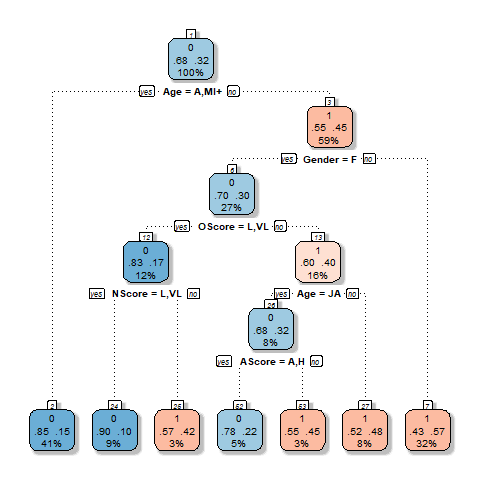
\includegraphics[height=7.5cm]{figuras/arvore_stimulating_pesada.png}}}%
    \caption{Visualização da árvore de decisão com função perda modificada para o grupo de drogas estimulantes.}
    \label{fig_DTStimulating_loss}
\end{figure}

Por fim, aplicou-se o método de poda sobre a árvore com função perda modificada. A árvore podada obtida corresponde a um modelo apenas com as variáveis \textbf{Idade (Age), Gênero (Gender), Abertura (OScore)}. Analisando-se as Tabelas \ref{resultadosdt_stimulating_podada} e \ref{matrizconfusaodt_stimulating_podada}, nota-se que, apesar de termos retirado duas variáveis do modelo, nenhuma das métricas de performance caiu consideravelmente, indicando que aqui o uso da árvore podada pode ser adequado. A árvore final pode ser observada na Figura \ref{fig_DTStimulating_podada}.

\begin{table}[H]
\centering
\begin{tabular}{||c|c|c|c||}
\hline
Conjunto & Acurácia & Sensibilidade & Especificidade \\ \hline
Treino & 68,86\% & 74,71\% & 66,05\% \\ \hline
Teste & 64,77\% & 74,72\% & 60,00\% \\ \hline
\end{tabular}
\caption{Métricas de performance da árvore de decisão para o grupo de drogas estimulantes.}
\label{resultadosdt_stimulating_podada}
\end{table}

\begin{table}[H]
\centering
\begin{tabular}{cc|c|c|c}
\cline{3-4}
 & & \multicolumn{2}{c|}{Valor Verdadeiro} & \\ \cline{3-4}
 & & Positivo & Negativo & \\ \cline{1-4}
\multicolumn{1}{|c|}{\multirow{2}{*}{\rotatebox[origin=c]{90}{Valor Previsto}}} & \multicolumn{1}{c|}{\rotatebox[origin=c]{90}{ Positivo }} & \multicolumn{1}{c|}{68} & 76 & \\ \cline{2-4}
\multicolumn{1}{|c|}{} & \multicolumn{1}{c|}{\rotatebox[origin=c]{90}{ Negativo }} & \multicolumn{1}{c|}{23} & 114 & \\ \cline{1-4}
\end{tabular}
\caption{Tabela de confusão do conjunto de teste da árvore de decisão podada para o grupo de drogas estimulantes.}
\label{matrizconfusaodt_stimulating_podada}
\end{table}

\begin{figure}[H]
    \centering
    \textbf{Árvore de Decisão Podada - Drogas Estimulantes}\par\medskip
    \subfloat{{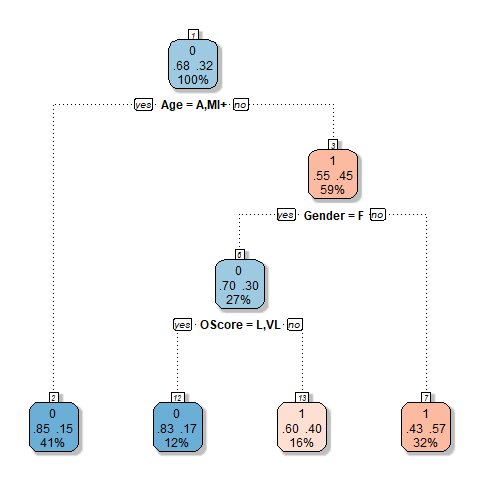
\includegraphics[height=8cm]{figuras/arvore_stimulating_podada.png}}}%
    \caption{Visualização da árvore de decisão podada para o grupo de drogas estimulantes.}
    \label{fig_DTStimulating_podada}
\end{figure}

% ---
% Finaliza a parte no bookmark do PDF, para que se inicie o bookmark na raiz
% ---
\bookmarksetup{startatroot}% 

\subsection{Comparativo dos Resultados}

Finalizada a aplicação dos métodos de regressão logística e de árvores de decisão para todas as drogas escolhidas, podemos analisar os resultados para comparar a performance dos métodos e procurar por padrões nos resultados. Um compilado dos resultados finais obtidos pode ser observado na Tabela \ref{tabela_resultados_com_var}. Os resultados para o álcool foram desprezados devido à péssima qualidade dos ajustes.

\begin{table}[H]
\centering
\addtolength{\leftskip}{-0.8cm}
\begin{tabular}{cccccccccc}
\hline
 & \multicolumn{4}{c}{\textbf{Regressão Logística}} & \multicolumn{4}{c}{\textbf{Árvore de Decisão}} &  &  &  \\
 & Acur. & Sens. & Especif.& Nº Var. & Acur. & Sens. & Especif. & Nº Var. &  \\ \hline
\textbf{Cannabis} &  &  &  &  &  &  &  &  & \\
Treino & 77,27\% & 71,41\% & 83,82\% & 6& 75,39\% & 74,02\% & 76,92\% & 4&  \\
Teste &  76,43\% &  75,00\% &  78,03\% & 6&  71,43\% &  71,62\%&  71,21\%& 4 &  \\ \hline
\textbf{Ecstasy} &  &  &  &  &  &  &  &  &  \\
Treino & 76,08\% & 68,65\% & 78,88\% & 6& 73,32\% & 76,20\% & 72,24\%  & 3&  \\
Teste &  77,14\% & 65,79\% & 81,37\% & 6& 74,64\% & 69,34\% & 76,47\% & 3 &  \\ \hline
\textbf{Estimulantes} &  &  &  &  &  &  &  &  &  \\
Treino & 72,74\% & 59,29\% & 79,22\% & 6& 68,86\%& 74,71\% & 66,05\% & 3 &  \\
Teste & 70,82\% & 63,74\% & 74,21\% & 6& 64,77\% & 74,72\% & 60,00\% & 3 &  \\ \hline
 &  &  &  &  &  &  &  &  &  \\
 &  &  &  &  &  &  &  &  & 
\end{tabular}
\caption{Acurácia, sensibilidade, especificidade e número de variáveis do modelo obtido para os métodos de regressão logística e árvore de decisão.}
\label{tabela_resultados_com_var}
\end{table}

A partir dos resultados da Tabela \ref{tabela_resultados_com_var}, é possível notar que os métodos aplicados possuem as suas particularidades. A regressão logística performa consistentemente melhor em termos de acurácia e de especificidade, enquanto a árvore de decisão em geral alcança resultados melhores para a sensibilidade e consegue gerar modelos mais parsimoniosos. Apesar disso, os resultados dos dois modelos ficaram consideravelmente próximos, sendo ambos válidos para serem aplicados nessa análise.

Além dessas questões, uma observação mais aprofundada dos problemas de classificação estudados nos permite avaliar a aplicabilidade desses modelos sobre distribuições desbalanceadas. As análises mais simples de serem realizadas foram as da droga cannabis, cuja distribuição era bem balanceada. Nos casos em que a distribuição das classes fica na faixa dos 70\% - 30\%, o que corresponde ao ecstasy e ao conjunto de drogas estimulantes, as modelagens precisaram levar em conta o uso de técnicas extras (uso de pesos/custos mais elevados para erros de classificação) para alcançar uma performance adequada. Por fim, no caso do álcool, em que temos uma amostra extremamente desbalanceada (com uma das classes tendo uma predominância de mais de 90\%), nenhum dos modelos se mostrou efetivo, evidenciando que existem situações onde os problemas pré-existentes no banco de dados não conseguem ser superados pelos algoritmos.

\subsection{Resultados por Atributo}

Além de analisarmos os resultados do ponto de vista dos métodos utilizados, podemos analisá-los da perspectiva dos atributos utilizados. Em outras palavras, podemos avaliar quais variáveis estavam presentes em cada modelo e quais dos seus níveis estão ligados ao uso de determinada droga. Um compilado da presença de cada uma das variáveis nos diferentes ajustes finais obtidos pode ser encontrado na Tabela \ref{tabela_resultados_atributos}. Devido a péssima qualidade do ajuste para o álcool, iremos desconsiderá-lo nessa análise e focar apenas nas drogas ilícitas.

\begin{table}[H]
\centering
\addtolength{\leftskip}{-0.8cm}
\begin{tabular}{cccccccccc}
\hline
 & Idade & Educação & Gênero & NScore & EScore & OScore & AScore & CScore &  \\ \hline
\textbf{Cannabis} &  &  &  &  &  &  &  &  &  \\
RL & X & X & X & X &  & X  & &X &  \\
DT & X &  & X &  &  & X & &X &  \\ \hline
\textbf{Ecstasy} &  &  &  &  &  &  &  &  &  \\
RL & X & X & X &  &  & X  & X &X &  \\
DT & X &  & X &  &  & X  & & &  \\ \hline
\textbf{Estimulantes} &  &  &  &  &  &  &  &  &  \\
RL & X & X & X &  &  & X  & X &X &  \\
DT & X &  & X &  &  & X  & & &  \\ \hline
 &  &  &  &  &  &  &  &  &  \\
 &  &  &  &  &  &  &  &  & 
\end{tabular}
\caption{Presença dos atributos na seleção de variáveis dos métodos de regressão logística e árvore de decisão.}
\label{tabela_resultados_atributos}
\end{table}

Analisando cada uma das variáveis de maneira isolada e levando em consideração todos os modelos gerados, podemos ter um panorama do perfil de usuário de drogas. Começando pelos indicadores sociais, temos que Idade costuma ser um fator relevante pois os mais jovens (entre 18 e 24 anos) possuem uma tendência mais elevada de serem usuários de drogas em comparação com os indivíduos de idade mais avançada, em especial considerando a faixa acima dos 45 anos. Da mesma forma, os homens aparecem como um grupo de maior risco, chegando a ter quase o dobro de chance de serem usuários de drogas do que as mulheres para algumas das drogas. É importante ressaltar, contudo, que jovens na faixa dos 18 aos 24 anos são maioria na amostra, o que pode interferir no resultado.

Educação já é um atributo de comportamento mais instável: ele aparece em todas as análises de regressão logística, mas em nenhum dos modelos finais das árvores de decisão. Nos casos em que ela aparece no modelo, a tendência indica que pessoas com um nível mais elevado de educação possuem uma chance significativamente menor de serem usuários de droga, em especial em comparação com as pessoas que abandoram a escola ou que não possuem nenhum diploma.

Em relação aos Scores do NEO-FFI-R, tem-se que os principais fatores são o OScore (Abertura) e o CScore (Conscienciosidade). Para o Score que mede a Abertura, temos que o uso de drogas está bastante relacionado com o fato de possuir um valor mais elevado (médio ou alto) nessa métrica. No caso da Conscienciosidade, o inverso ocorre: o uso de drogas está ligado com valores baixos de Score nessa métrica.

Os demais Scores já possuem uma presença mais esporádica: EScore, a medida associado à Extroversão, nem sequer aparece nos modelos finais, sendo portanto uma variável irrelevante para determinar o uso de drogas. Já o Score de Socialização (AScore), quando aparece, indica que indivíduos com pontuações baixas nessa categoria possuem uma maior tendência a serem usuários de drogas. Por fim, o score de Neuroticismo (NScore) aparece em apenas um dos modelos e possui um comportamento menos definido do que os demais: a classe com maior chance de uso de drogas é a com pontuações de valores médios. Essa instabilidade é justificada em boa parte pela própria distribuição dos dados: observando novamente as Figuras \ref{comp1}, \ref{comp2} e \ref{comp3}, nota-se que esse Score é o que mais foge da distribuição normal, estando extremamente concentrado em torno dos valores mais baixos.



% ----------------------------------------------------------
% Conclusão
% ----------------------------------------------------------
\section{Considerações Finais}

Este trabalho teve como objetivo observar características associadas ao uso de drogas específicas, utilizado para isto as técnicas de classificação de regressão logística e de árvores de decisão. 
Em uma análise mais detalhada dos métodos, foi possível notar que os modelos ajustados apresentaram acurácia e especificidade levemente superiores na modelagem por regressão e acima de 70\% para as drogas cannabis e ecstasy, mantendo a performance quando comparados treino e teste. Para as drogas estimulantes, a árvore de decisão foi que apresentou pior desempenho com acurácia e especificidade respectivamente de 68,68\% e 66,05\% no treino e 64,77\% e 60,05\% no teste. Em relação a sensibilidade, as árvores de decisão apresentaram resultados ligeiramente superiores a regressão logística. Pode-se concluir que os modelos obtidos, tanto na regressão logística, quanto nas árvores de decisão, são satisfatórios na classificação de usuários para as drogas cannabis, ecstasy e para o grupo de drogas estimulantes. Para o álcool não foi possível estimar um modelo adequado, dada a proporção da amostra obtida.

A indicação final é a utilização dos modelos que classifiquem melhor em relação a sensibilidade de forma a não prejudicar a acurácia, pois estamos realizando análises com objetivo inferencial e com foco na modelagem dos usuários de drogas. Dessa forma, os melhores modelos seriam o modelo de regressão para cannabis, enquanto ecstasy e o grupo de drogas estimulantes são ajustados de maneira mais adequada pela árvore de decisão. Contudo, é importante ressaltar que os modelos tiveram performances consideravelmente similares, e que escolher um deles em detrimento do outro não acarreta em grandes perdas de performance.

Em relação ao perfil dos usuários de drogas, as variáveis idade, gênero e Oscore se mostraram como as mais importantes, entrando em todos os modelos propostos. Considerando os diferentes modelos, o perfil geral do usuário de drogas que observou-se caracteriza esses indivíduos como sendo jovens, predominantemente homens e com nível educacional mais baixo. Quanto aos traços de personalidade do NEO-FFI-R, os resultados indicam que o consumo de drogas está ligado com baixos escores de Conscienciosidade (C) e de Socialização (A) e com altos escores de Abertura(O). Esses achados estão de acordo com a literatura sobre o assunto \cite{fehrman2015}.

Por fim, é importante ressaltar que os dados coletados podem estar viesados, dado a estratégia adotada de amostragem não probabilística, impossibilitando a generalização dos resultados para a população. Ainda assim, os resultados obtidos são interessantes tanto para a geração de \emph{insights} para possíveis ações de prevenção, quanto para próximas pesquisas.

Sugere-se como análises futuras a exploração de tais problemas de classificação para as demais drogas que não foram abordadas nesse estudo, de tal forma a termos um espectro mais completo do perfil de usuários de diferentes drogas. Além disso, a repetição dessas mesmas análises em amostra não viesadas dos dados é desejável, de tal forma a nos permitir determinar com mais clareza o quanto cada variável de fato influencia no uso de drogas.



% ----------------------------------------------------------
% Referências bibliográficas
% ----------------------------------------------------------
\bibliography{referencias}


% ----------------------------------------------------------
% Glossário
% ----------------------------------------------------------
%
% Há diversas soluções prontas para glossário em LaTeX. 
% Consulte o manual do abnTeX2 para obter sugestões.
%
%\glossary

% ----------------------------------------------------------
% Apêndices
% ----------------------------------------------------------

\break



\newgeometry{margin=2.0cm}

\pagestyle{empty}
\begin{landscape}
\begin{table}[h!]
\centering
\addtolength{\leftskip}{-0.4cm}
\begin{tabular}{cccccccccc}
\hline
\multicolumn{10}{c}{\textbf{Apêndice A - Tabela de Frequências}} \\
\hline
 &  & \multicolumn{2}{c}{\textbf{Cannabis}} & \multicolumn{2}{c}{\textbf{Ecstasy}} & \multicolumn{2}{c}{\textbf{Álcool}} & \multicolumn{2}{c}{\textbf{Grupo de Estimulantes}} \\
 & \begin{tabular}[c]{@{}c@{}}\textbf{Amostra}\\ n=1877\end{tabular} & \begin{tabular}[c]{@{}c@{}}Usuário\\ 991 (53\%)\end{tabular} & \begin{tabular}[c]{@{}c@{}}Não Usuário\\ 886 (47\%)\end{tabular} & \begin{tabular}[c]{@{}c@{}}Usuário\\ 513 (27\%)\end{tabular} & \begin{tabular}[c]{@{}c@{}}Não Usuário\\ 1364 (73\%)\end{tabular} & \begin{tabular}[c]{@{}c@{}}Usuário\\ 1742 (93\%)\end{tabular} & \begin{tabular}[c]{@{}c@{}}Não Usuário\\ 135 (7\%)\end{tabular} & \begin{tabular}[c]{@{}c@{}}Usuário\\ 609 (32\%)\end{tabular} & \begin{tabular}[c]{@{}c@{}}Não Usuário\\ 1268 (68\%)\end{tabular} \\ \cline{1-10}
\textbf{Sexo} & \multicolumn{1}{l}{} & \multicolumn{1}{l}{} & \multicolumn{1}{l}{} & \multicolumn{1}{l}{} & \multicolumn{1}{l}{} & \multicolumn{1}{l}{} & \multicolumn{1}{l}{} & \multicolumn{1}{l}{} & \multicolumn{1}{l}{} \\
Feminino & 937 & 359 (38\%) & 578 (62\%) & 166 (18\%) & 771 (82\%) & 873 (93\%) & 64 (7\%) & 210 (22\%) & 727 (78\%) \\
Masculino & 940 & 632 (67\%) & 308 (33\%) & 347 (37\%) & 593 (63\%) & 869 (92\%) & 71 (8\%) & 399 (42\%) & 541 (58\%) \\ \cline{1-10}
\textbf{Idade} & \multicolumn{1}{l}{} & \multicolumn{1}{l}{} & \multicolumn{1}{l}{} & \multicolumn{1}{l}{} & \multicolumn{1}{l}{} & \multicolumn{1}{l}{} & \multicolumn{1}{l}{} & \multicolumn{1}{l}{} & \multicolumn{1}{l}{} \\
18-24 & 637 & 530 (83\%) & 107 (17\%) & 321 (50\%) & 316 (50\%) & 611 (96\%) & 26 (4\%) & 329 (52\%) & 308 (48\%) \\
25-34 & 480 & 237 (49\%) & 243 (51\%) & 126 (26\%) & 354 (74\%) & 453 (94\%) & 27 (6\%) & 167 (35\%) & 313 (65\%) \\
35-44 & 355 & 122 (34\%) & 233 (66\%) & 44 (12\%) & 311 (88\%) & 321 (90\%) & 34 (10\%) & 66 (19\%) & 289 (81\%) \\
45+ & 405 & 102 (25\%) & 303 (75\%) & 22 (5\%) & 383 (95\%) & 357 (88\%) & 48 (12\%) & 47 (12\%) & 358 (88\%) \\ \cline{1-10}
\textbf{Educação} & \multicolumn{1}{l}{} & \multicolumn{1}{l}{} & \multicolumn{1}{l}{} & \multicolumn{1}{l}{} & \multicolumn{1}{l}{} & \multicolumn{1}{l}{} & \multicolumn{1}{l}{} & \multicolumn{1}{l}{} & \multicolumn{1}{l}{} \\
LS* & 254 & 148 (58\%) & 106 (42\%) & 70 (28\%) & 184 (72\%) & 231 (92\%) & 23 (8\%) & 87 (34\%) & 167 (66\%) \\
Curso profissionalizante & 270 & 118 (44\%) & 152 (56\%) & 51 (19\%) & 219 (81\%) & 244 (90\%) & 26 (10\%) & 70 (26\%) & 200 (74\%) \\
College/Univ. (sem diploma) & 503 & 405 (81\%) & 98 (19\%) & 230 (46\%) & 273 (54\%) & 470 (93\%) & 33 (7\%) & 253 (50\%) & 250 (50\%) \\
Diploma de graduação & 478 & 202 (42\%) & 276 (58\%) & 100 (21\%) & 378 (79\%) & 444 (93\%) & 34 (7\%) & 123 (26\%) & 355 (74\%) \\
Diploma mestrado ou doutorado & 372 & 118 (32\%) & 254 (68\%) & 62 (17\%) & 310 (83\%) & 353 (95\%) & 19 (5\%) & 76 (20\%) & 296 (80\%) \\ \cline{1-10}
\textbf{País} & \multicolumn{1}{l}{} & \multicolumn{1}{l}{} & \multicolumn{1}{l}{} & \multicolumn{1}{l}{} & \multicolumn{1}{l}{} & \multicolumn{1}{l}{} & \multicolumn{1}{l}{} & \multicolumn{1}{l}{} & \multicolumn{1}{l}{} \\
Reino Unido & 1044 & 307 (29\%) & 737 (71\%) & 159 (15\%) & 885 (85\%) & 969 (93\%) & 75 (7\%) & 162 (16\%) & 882 (84\%) \\
Estados Unidos & 551 & 482 (87\%) & 69 (13\%) & 242 (44\%) & 309 (56\%) & 513 (93\%) & 38 (7\%) & 314 (57\%) & 237 (43\%) \\
Outros & 282 & 202 (72\%) & 80 (28\%) & 112 (40\%) & 170 (60\%) & 260 (92\%) & 22 (8\%) & 133 (47\%) & 149 (53\%) \\ \cline{1-10}
\textbf{Grupo Étnico} & \multicolumn{1}{l}{} & \multicolumn{1}{l}{} & \multicolumn{1}{l}{} & \multicolumn{1}{l}{} & \multicolumn{1}{l}{} & \multicolumn{1}{l}{} & \multicolumn{1}{l}{} & \multicolumn{1}{l}{} & \multicolumn{1}{l}{} \\
Brancos & 1715 & 912 (53\%) & 803 (47\%) & 466 (27\%) & 1249 (73\%) & 1600 (93\%) & 115 (7\%) & 552 (32\%) & 1163 (68\%) \\
Negros & 33 & 8 (24\%) & 25 (76\%) & 3 (9\%) & 30 (91\%) & 25 (76\%) & 8 (24\%) & 5 (15\%) & 28 (85\%) \\
Outros & 129 & 71 (55\%) & 58 (45\%) & 44 (34\%) & 85 (66\%) & 117 (91\%) & 12 (9\%) & 52 (40\%) & 77 (60\%) \\ \cline{1-10}
*Deixou a escola (\emph{left school})  &
\end{tabular}
\caption{Frequências das variáveis sexo, idade, educação, país e grupo étnico nas amostras de interesse.}
\label{tabela_frequencias}
\end{table}
\end{landscape}
\pagestyle{plain}

\restoregeometry

\break

\newgeometry{margin=2.0cm}

\pagestyle{empty}
\begin{landscape}
\begin{table}[h!]
\centering
%\addtolength{\leftskip}{-1.0cm}
\begin{tabular}{cccccccccc}
\hline
\multicolumn{10}{c}{\textbf{Apêndice B - Tabela de Frequências}} \\
\hline
 &  & \multicolumn{2}{c}{\textbf{Cannabis}} & \multicolumn{2}{c}{\textbf{Ecstasy}} & \multicolumn{2}{c}{\textbf{Álcool}} & \multicolumn{2}{c}{\textbf{Grupo de Estimulantes}} \\
 & \begin{tabular}[c]{@{}c@{}} \textbf{Amostra}\\ 1885\end{tabular} & \begin{tabular}[c]{@{}c@{}}Usuário\\  991 (53\%)\end{tabular} & \begin{tabular}[c]{@{}c@{}}Não Usuário\\ 886 (47\%)\end{tabular} & \begin{tabular}[c]{@{}c@{}}Usuário\\ 513 (27\%)\end{tabular} & \begin{tabular}[c]{@{}c@{}}Não Usuário\\ 1364 (73\%)\end{tabular} & \begin{tabular}[c]{@{}c@{}}Usuário\\ 1742 (93\%)\end{tabular} & \begin{tabular}[c]{@{}c@{}}Não Usuário\\ 135 (7\%)\end{tabular} & \begin{tabular}[c]{@{}c@{}}Usuário\\ 609 (32\%)\end{tabular} & \begin{tabular}[c]{@{}c@{}}Não Usuário\\ 1268 (68\%)\end{tabular}  \\ \hline
\textbf{NScore} &  &  &  &  &  &  &  &  &  \\
Muito baixo & 864 & 404 (47\%) & 460 (53\%) & 221 (26\%) & 643 (74\%) & 803 (93\%) & 61 (7\%) & 226 (26\%) & 638 (74\%) \\
Baixo & 655 & 351 (54\%) & 304 (46\%) & 174 (27\%) & 481 (73\%) & 611 (93\%) & 44 (7\%) & 224 (34\%) & 431 (66\%) \\
Médio & 321 & 215 (67\%) & 106 (33\%) & 108 (34\%) & 213 (66\%) & 293 (91\%) & 28 (9\%) & 144 (45\%) & 177 (55\%) \\
Alto & 37 & 21 (57\%) & 16 (43\%) & 10 (27\%) & 27 (73\%) & 35 (95\%) & 2 (5\%) & 15 (41\%) & 22 (59\%) \\ \hline
\textbf{EScore} &  &  &  &  &  &  &  &  &  \\
Muito baixo & 428 & 254 (60\%) & 174 (40\%) & 111 (26\%) & 317 (74\%) & 396 (93\%) & 32 (7\%) & 160 (37\%) & 268 (63\%) \\
Baixo & 1011 & 499 (49\%) & 512 (51\%) & 254 (25\%) & 757 (75\%) & 932 (92\%) & 79 (8\%) & 296 (29\%) & 715 (71\%) \\
Médio & 424 & 227 (54\%) & 197 (46\%) & 141 (33\%) & 283 (67\%) & 400 (94\%) & 24 (6\%) & 145 (34\%) & 279 (66\%) \\
Alto & 14 & 11 (79\%) & 3 (21\%) & 7 (50\%) & 7 (50\%) & 14 (100\%) & 0 (0\%) & 8 (57\%) & 6 (43\%) \\ \hline
\textbf{OScore} &  &  &  &  &  &  &  &  &  \\
Muito baixo & 100 & 19 (19\%) & 81 (81\%) & 13 (13\%) & 87 (87\%) & 93 (93\%) & 7 (7\%) & 19 (19\%) & 81 (81\%) \\
Baixo & 657 & 232 (35\%) & 425 (65\%) & 102 (16\%) & 555 (84\%) & 604 (92\%) & 53 (8\%) & 146 (22\%) & 511 (78\%) \\
Médio & 947 & 597 (63\%) & 350 (37\%) & 313 (33\%) & 634 (67\%) & 884 (93\%) & 63 (7\%) & 352 (37\%) & 595 (63\%) \\
Alto & 173 & 143 (83\%) & 30 (17\%) & 85 (49\%) & 88 (51\%) & 161 (93\%) & 12 (7\%) & 92 (53\%) & 81 (47\%) \\ \hline
\textbf{AScore} &  &  &  &  &  &  &  &  &  \\
Muito baixo & 188 & 119 (63\%) & 69 (37\%) & 67 (36\%) & 121 (64\%) & 178 (94\%) & 10 (6\%) & 99 (53\%) & 89 (47\%) \\
Baixo & 907 & 509 (56\%) & 398 (44\%) & 267 (29\%) & 640 (71\%) & 842 (93\%) & 65 (7\%) & 315 (35\%) & 592 (65\%) \\
Médio & 736 & 346 (47\%) & 390 (53\%) & 172 (23\%) & 564 (77\%) & 681 (93\%) & 55 (7\%) & 187 (25\%) & 549 (75\%) \\
Alto & 46 & 17 (37\%) & 29 (63\%) & 7 (15\%) & 39 (85\%) & 41 (89\%) & 5 (11\%) & 8 (17\%) & 38 (83\%) \\ \hline
\textbf{CScore} &  &  &  &  &  &  &  &  &  \\
Muito baixo & 319 & 237 (74\%) & 82 (26\%) & 124 (39\%) & 195 (61\%) & 300 (94\%) & 19 (6\%) & 166 (52\%) & 153 (48\%) \\
Baixo & 866 & 505 (58\%) & 361 (42\%) & 264 (30\%) & 602 (70\%) & 809 (93\%) & 57 (7\%) & 303 (35\%) & 563 (65\%) \\
Médio & 667 & 237 (36\%) & 430 (64\%) & 119 (18\%) & 548 (82\%) & 609 (91\%) & 58 (9\%) & 131 (20\%) & 536 (80\%) \\
Alto & 25 & 12 (48\%) & 13 (52\%) & 6 (24\%) & 19 (76\%) & 24 (96\%) & 1 (4\%) & 9 (36\%) & 16 (64\%) \\ \hline
\end{tabular}
\caption{Frequências das variáveis relacionadas aos treços de personalidade (\emph{Scores}) nas amostras de interesse.}
\label{tabela_scores}
\end{table}
\end{landscape}
\pagestyle{plain}

\restoregeometry


% ----------------------------------------------------------
% Anexos
% ----------------------------------------------------------
%\cftinserthook{toc}{AAA}
%\anexos
%\begin{anexosenv}
%
%\chapter{Anexo}
%
%\lipsum[31]
%\end{anexosenv}


\section*{\textbf{Apêndice C}}

\begin{table}[H]											
\centering											
\begin{tabular}{|l|l|}											
\hline
Age25-34	&	0.36	\\	\hline
Age35-44	&	0.17	\\	\hline
Age45+	&	0.1	\\	\hline
GenderMale	&	2.48	\\	\hline
EducationLeft	school	&	3.99	\\	\hline
EducationProfessional	certificate/	diploma	&	2.15	\\	\hline
EducationSome	college	or	university,	no	certificate	or	degree	&	3.5	\\	\hline
EducationUniversity	degree	&	1.59	\\	\hline
NScoreHigh	&	0.46	\\	\hline
NScoreLow	&	0.72	\\	\hline
NScoreVeryLow	&	0.65	\\	\hline
CScoreHigh	&	1.09	\\	\hline
CScoreLow	&	1.89	\\	\hline
CScoreVeryLow	&	2.93	\\	\hline
OScoreHigh	&	2.48	\\	\hline
OScoreLow	&	0.34	\\	\hline
OScoreVeryLow	&	0.12	\\	\hline
\end{tabular}											
\caption{Odds Ratio da	Regressão	Logística	para	a	Cannabis}					
\label{oddsratio_reglog_cannabis}											
\end{table}											

\begin{table}[H]										
\centering										
\begin{tabular}{|l|r|}										
\hline										
Age25-34	&	0.51	\\	\hline						
Age35-44	&	0.17	\\	\hline						
Age45+	&	0.09	\\	\hline						
GenderMale	&	1.91	\\	\hline						
EducationLeft	school	&	1.55	\\	\hline					
EducationProfessional	certificate/	diploma	&	1.47	\\	\hline				
EducationSome	college	or	university,	no	certificate	or	degree	&	1.64	\\	\hline
EducationUniversity	degree	&	1.1	\\	\hline					
CScoreHigh	&	0.76	\\	\hline						
CScoreLow	&	1.34	\\	\hline						
CScoreVeryLow	&	1.31	\\	\hline						
AScoreHigh	&	0.58	\\	\hline						
AScoreLow	&	1.27	\\	\hline						
AScoreVeryLow	&	1.57	\\	\hline						
OScoreHigh	&	1.95	\\	\hline						
OScoreLow	&	0.5	\\	\hline						
OScoreVeryLow	&	0.56	\\	\hline						
\end{tabular}										
\caption{Odds Ratio	Regressão	Logística	para	o	Ecstasy}				
\label{oddsratio_reglog_ecstasy}										
\end{table}										


\begin{table}[H]											
\centering											
\begin{tabular}{|l|r|}											
\hline											
Age25-34	&	0.79	\\	\hline							
Age35-44	&	0.36	\\	\hline							
Age45+	&	0.18	\\	\hline							
GenderMale	&	1.82	\\	\hline							
EducationLeft	school	&	1.62	\\	\hline						
EducationProfessional	certificate/	diploma	&	1.48	\\	\hline					
EducationSome	college	or	university,	no	certificate	or	degree	&	1.78	\\	\hline
EducationUniversity	degree	&	1.06	\\	\hline						
CScoreHigh	&	1.4	\\	\hline							
CScoreLow	&	1.47	\\	\hline							
CScoreVeryLow	&	2.61	\\	\hline							
AScoreHigh	&	0.68	\\	\hline							
AScoreLow	&	1.39	\\	\hline							
AScoreVeryLow	&	2.55	\\	\hline							
OScoreHigh	&	1.73	\\	\hline							
OScoreLow	&	0.54	\\	\hline							
OScoreVeryLow	&	0.51	\\	\hline							
\end{tabular}											
\caption{Odds Ratio	da	Regressão	Logística	para	o	grupo	de	Drogas	Estimulantes}		
\label{oddsratio_reglog_stimulants}											
\end{table}											


\end{document}